\chapter{Theoretical background}
\label{ch:2}
\paragraph{}
This chapter reviews the fundamental physics theory and machine learning concepts underpinning this thesis.
The chapter begins with an overview of lattice vibrations, covering topics from the calculation of force constants to thermal properties, with a focus on \textbf{Anharmonic Phonons}.
Section \ref{sec:2.2} provides a concise introduction to \textbf{Density Functional Theory (DFT)}, the electronic structure theory typically used for calculating force constants.
In section \ref{sec:2.3}, the \textbf{Gaussian Process (GP)} model is introduced as a surrogate tool for predicting lattice force constants based on DFT results. This section also highlights how incorporating physics-informed constraints into the GP model can enhance its predictions.
Section \ref{sec:2.4}, \textbf{Inductive Bias: Equivariant Representations}, explores the integration of physical principles into machine learning models. Among the widely used equivariant representations, the O(3) representation, as used in e.g. \textbf{Atomic Cluster Expansions (ACE)}, is described in detail in section \ref{sec:2.5}. The utility of the ACE representation extends beyond lattice force constant predictions, as these are also a useful inductive bias for modelling transfer integrals in molecular dimers.
Finally, section \ref{sec:2.6} provides a brief introduction to electronic \textbf{Transfer Integrals} as used to model electronic properties of organic semiconductors, concluding the chapter.

%This chapter begins with revisiting the fundamental concept of Gaussian distributions and Bayesian inference.A Gaussian process (GP) model, i.e. GP regression, is introduced in section \ref{sec:2.2}. This section also provides the application to calculates potential energy surfaces (PESs) of atomic environment from input PESs. To allow a GP model conditioned (trained) on energies and forces of atomic environment may require the modification of a GP model by taking derivatives of a GP \textit{kernel} (a covariance function). In the last section (\ref{sec:2.3}), the full derivation and covariance matrix construction required for training the derivative GP model are demonstrated.

%\section{Symmetry and Group Theory}
%This section reviews the symmetry and group theory in quantum chemistry. Firstly, we start with discussing the discrete symmetry and point groups in an atomic environment and spectroscopy. Subsequently, in the sub-atomic environment (like electrons in orbitals), the continuous symmetry and corresponding Lie groups need to be considered.
\newpage

\section{Phonons and (an)harmonic potentials} \label{sec:2.1}
\begin{figure}
\centering

\includegraphics[width=1\textwidth]{Figure/Chapter 2/2D-Chain.jpg}
\caption{\label{fig:2.1}
The infinite one-dimensional diatomic chain consists of an infinite number of unit cells. In the $l^{\text{th}}$ unit cell, two atoms with masses $m_1$ (yellow) and $m_2$ (green) are labeled by $\kappa = 1$ and $\kappa = 2$, respectively. %Each atom vibrates around its equilibrium position, $\mathbf{R}^0_{l,1}$ and $\mathbf{R}^0_{l,2}$, with displacements $u_{l,1}$ and $u_{l,2}$, caused by harmonic interactions with neighboring atoms.
}
\end{figure}
\paragraph{}
This section introduces the foundational concepts of lattice vibrations in crystalline solids, focusing on both harmonic and anharmonic descriptions. It is divided into two subsections: Subsection \ref{subsec:2.1.1}, which discusses the calculation of lattice force constants using finite difference methods, and Subsection \ref{subsec:2.1.2}, which delves into the theory of phonons and lattice thermal conductivity derived from these force constants.

\subsection{Lattice Force Constants} \label{subsec:2.1.1}

In crystalline materials, atoms are assumed to vibrate around their equilibrium positions, $\mathbf{R}^0_{l\kappa}$, with displacements $\mathbf{u}_{l\kappa} = \mathbf{R}_{l\kappa}-\mathbf{R}^0_{l\kappa}$, where $\kappa$ and $l$ denote the $\kappa^{\text{th}}$ atom in the $l^{\text{th}}$ unit cell.
As an example, Fig. \ref{fig:2.1} illustrates an infinite diatomic chain.
To derive the lattice vibrational properties, we begin by examining the Hamiltonian of the system, expressed as:
\begin{equation}
\label{equ:2.1}
         \mathcal{H} = \sum_{l\kappa}m_{\kappa}\left(\frac{d{\mathbf{u}}_{l\kappa}}{dt}\right)^{2} + \Phi,       
\end{equation}
where $\Phi$ represents the lattice potential energy. The potential term can be expanded using a Taylor series around the equilibrium positions $\mathbf{R}^0_{l\kappa}$.
Following \cite{Togo2015, Togo2015-qf, Phonopy_toolkit, phonopy}, this expansion is expressed as:
\begin{equation}
\label{equ:2.2}
\begin{split}
        \Phi =\: \Phi^{(0)} &+ \sum_{\alpha l\kappa} \Phi^{(1)}_{\alpha l\kappa} \, u^{\alpha}_{l\kappa} \\
            & + \frac{1}{2} \sum_{\alpha l \kappa} \sum_{\beta l' \kappa'} \Phi^{(2)}_{\alpha l\kappa,\;\beta l'\kappa'} \, u^{\alpha}_{l\kappa} \cdot u^{\beta}_{l'\kappa'} \\
            & + \frac{1}{3!} \sum_{\alpha l \kappa} \sum_{\beta l' \kappa'} \sum_{\gamma l''\kappa''} \Phi^{(3)}_{\alpha l\kappa,\;\beta l'\kappa',\;\gamma l''\kappa''} \, u^{\alpha}_{l\kappa} \cdot u^{\beta}_{l'\kappa'} \cdot u^{\gamma}_{l''\kappa''} \\
            &+ \cdots,
\end{split}
\end{equation}
where $\alpha$, $\beta$, and $\gamma$ represent the Cartesian coordinate directions and $\Phi^{(n)}$ is the $n^{\text{th}}$-order force constants.
The zeroth-order term corresponds to the potential energy at equilibrium.
The first-order force constant of the potential energy vanishes at equilibrium positions because $\Phi^{(1)}_{\alpha l\kappa} = \frac{\partial \Phi}{\partial u^{\alpha}_{l \kappa}}\bigg|_{\mathbf{u}=0}$ represents the force, which is always zero at the equilibrium positions of the system.
The harmonic (second-order) force constants, which describe the vibrational properties within the harmonic approximation, can be derived in a similar manner to  $\Phi^{(1)}$, as: 
\begin{equation}
\label{equ:2.3}
\begin{split}
        \Phi^{(2)}_{\alpha l \kappa,\;\beta l' \kappa'} = \frac{\partial^{2} \Phi}{\partial u^{\alpha}_{l \kappa} \partial u^{\beta}_{l'\kappa'}} \bigg|_{\mathbf{u}=0}.
\end{split}
\end{equation}
Terms beyond the harmonic approximation represent anharmonic contributions.
The cubic anharmonic (third-order) force constant, essential for collecting vibrational properties, is given by:
\begin{equation}
\label{equ:2.4}
\begin{split}
        \Phi^{(3)}_{\alpha l \kappa,\;\beta l' \kappa',\;\gamma l''\kappa''} = \frac{\partial^{3} \Phi}{\partial u^{\alpha}_{l \kappa} \partial u^{\beta}_{l'\kappa'} \partial u^{\gamma}_{l''\kappa''}} \bigg|_{\mathbf{u}=0}.
\end{split}
\end{equation}
%These anharmonic terms are crucial for accurately capturing the corrections beyond the harmonic approximation.
\begin{figure}
\centering

\includegraphics[width=1\textwidth]{Figure/Chapter 2/FDM.jpg}
\caption{\label{fig:2.2}
Schematic representation of harmonic and anharmonic force interactions in a lattice. %The left panel illustrates a harmonic interaction, where the force $F_\alpha(A)$ on atom $A$ is proportional to the displacement $u^\beta(B)$ of atom $B$. The right panel demonstrates an anharmonic interaction, where additional contributions from the displacement $u^\gamma(C)$ of a third atom $C$ affect the force on atom $A$, introducing higher-order corrections to the interaction potential.
}
\end{figure}
Equations (\ref{equ:2.3}) and (\ref{equ:2.4}) can be calculated using the Finite Difference Method (FDM). 
In this approach, the harmonic force constant (correlating atom $A$ and $B$) is determined by displacing atom $B$ by $u^\beta(B)$ and calculating the corresponding force $F_\alpha(A)$ acting on atom $A$, as illustrated in the left panel of Figure \ref{fig:2.2}.
Generally, this involves generating a displaced crystal structure and using it as input for electronic structure calculations, such as Density Functional Theory (DFT), which will be discussed in Section~\ref{sec:2.2}.
The resulting forces acting on atoms in the structure are then obtained via the Hellman–Feynman theorem from these calculations.
The harmonic force constant correlation between $A$ and $B$ is evaluated as follows:
\begin{equation}
\label{equ:2.5}
\begin{split}
        \Phi^{(2)}_{\alpha\beta}(A,\;B) = -\frac{F_{\alpha}(A)}{u^\beta(B)}.
\end{split}
\end{equation}

At equilibrium the net force on each atom vanishes (\(F_\alpha(A)=0\)), so the reference force at the undisplaced geometry cancels.  
Only the perturbed force appears in Eq.~(\ref{equ:2.5}), which explains the absence of an explicit “difference” term.  
In practice, a centred finite difference scheme is usually employed—displacing atom $B$ by \(+\!u^\beta(B)\) and \(-\!u^\beta(B)\)—to symmetrise the calculation about the equilibrium position.  
This cancels odd-order truncation errors and yields a more accurate \(\mathcal{O}(h^2)\) estimate of the force constants compared with forward or backward differences.

This centred finite difference pratically requires moving each atom a small displacement separately in $x, y, z$ , resulting in $\textbf{3N}$ independent displacements. For each displacement, the forces on all $3N$ atomic degrees of freedom must be evaluated, yielding a full $3N \times 3N$ force constant matrix. Using central finite differences, this requires $\textbf{6N}$ total force evaluations (two per displacement), leading to $\textbf{9N}^2$ distinct elements in the force constant matrix~\cite{kittel2005}. (Typically, these forces are obtained from an electronic structure method, such as density functional theory.)

For the cubic anharmonic force constants, a similar procedure is employed. This requires the simultaneous displacement of two atoms (e.g., atoms $B$ and $C$), while the resulting force acting on a third atom (e.g., atom $A$) is calculated, as depicted in the right panel of Figure~\ref{fig:2.2}. 

These calculations follow the same electronic structure calculation procedure as for the harmonic force constants, enabling the numerical determination of the cubic anharmonic force constants, expressed as:
\begin{equation}
\label{equ:2.6}
\begin{split}
        \Phi^{(3)}_{\alpha\beta\gamma}(A,\;B,\;C) = -\frac{F_\alpha(A)}{u^\beta(B)u^\gamma(C)}.
\end{split}
\end{equation}
The process of evaluating them through central finite differences requires the displacement of all pairs of atoms \( (B, C) \) in all Cartesian directions \( (\beta, \gamma) \), and the subsequent recording of the change in force on atom \( A \). Consequently, \( \textbf{9N}^2 \) distinct displacement pairings are generated, each necessitating four force evaluations, resulting in a total of \( \textbf{36N}^2 \) required force calculations. The third-order force constant tensor that results is significantly more expensive than the harmonic case due to the presence of \( \textbf{27N}^3 \) elements.

The computational cost arises from the extensive number of force evaluations (CPU time) required to generate the tensor and the considerable memory required for storing all those \(27N^3\) independent elements. 
Thus, calculations of third-order force constants increase combinatorially with system size and are far more resource-intensive than their harmonic equivalents.

\subsection{Phonon Calculations} \label{subsec:2.1.2}

Phonons are quantised periodic vibrations that describe the collective motion of atoms in a crystalline material. Their study is essential for understanding vibrational, thermal, and electrical transport properties in solids.
Phonon calculations begin with the construction of the dynamical matrix using harmonic force constants and solving the equations of motion for the lattice vibrations.


In the harmonic approximation, the potential energy of the lattice, Eq. (\ref{equ:2.2}), is expanded to the second order around the equilibrium positions. 
The equation of motion for the displacement of atoms is given by:
\begin{equation}
\label{equ:2.7}
    \begin{split}
        m_{\kappa}\frac{\partial^{2} u^{\alpha}_{l\kappa}(t)}{\partial t^{2}}=-\sum_{\beta l' \kappa'} \Phi^{(2)}_{\alpha l\kappa,\;\beta l'\kappa'}u^{\beta}_{l'\kappa'},
    \end{split}
\end{equation}
where $m_{\kappa}$ is the mass of the $\kappa^{\text{th}}$ atom in the $l^{\text{th}}$ unit cell.
%The atom displaces in $\alpha$ Cartesian direction by $u^{\alpha}_{l\kappa}$.
%$\Phi^{(2)}_{\alpha l\kappa,\;\beta l'\kappa'}$ are the harmonic force constants correlating between two atoms.

Due to the periodic boundary conditions of a crystal structure, the atomic displacements can be expressed as plane waves \cite{ziman_2007,kantorovich_2004}:
\begin{equation}
\label{equ:2.8}
    \begin{split}
        u^{\alpha}_{l\kappa}(t)= \sum_{j}\epsilon^{\alpha}_{\kappa,\;j}(\mathbf{q})\:\textbf{e}^{-i\left(\mathbf{q}\cdot\mathbf{R}^{0}_{\kappa l}-\omega_{j}(\mathbf{q})t\right)}.
    \end{split}
\end{equation}

In this expression, $\omega_{j}(\mathbf{q})$ is the phonon frequency associated with the $j^{\text{th}}$ phonon mode characterised by the wave vector $\mathbf{q}$.
The plane wave amplitude $\epsilon^{\alpha}_{\kappa,\;j}(\mathbf{q})$ represents the phonon polarisation in the $\alpha^{\text{th}}$ Cartesian direction. 
Substituting this expression into equation (\ref{equ:2.7}) leads to the dynamical matrix $\mathbf{D}$ eigenvalue problem:
\begin{equation}
\label{equ:2.9}
    \begin{split}
        \omega^{2}_{j}(\mathbf{q})\;\epsilon^{\alpha}_{\kappa,\;j}(\mathbf{q}) =  \sum_{\beta\;\kappa'}D_{\alpha\beta,\;\kappa\kappa'}(\mathbf{q})\;\epsilon^{\beta}_{\kappa',\;j}(\mathbf{q}),
    \end{split}
\end{equation}
where $D_{\alpha\beta,\;\kappa\kappa'}(\mathbf{q})$ is the discrete Fourier transform of the harmonic force constants \footnote{The translational symmetry, i.e. setting $l=0$, can be used to simplify Eq. (\ref{equ:2.10}) more symmetric, which appears in \cite{wallace_1998}.}, defined as:
\begin{equation}
\label{equ:2.10}
    \begin{split}
        D_{\alpha\beta,\;\kappa\kappa'}(\mathbf{q}) =  \sum_{l'}\frac{1}{\sqrt{m_{(\kappa)}m_{(\kappa')}}}\Phi^{(2)}_{\alpha l\kappa,\;\beta l'\kappa'}\:\textbf{e}^{i\mathbf{q}\cdot\left(\mathbf{R}^{0}_{\kappa' l'}-\mathbf{R}^{0}_{\kappa l}\right)}.
    \end{split}
\end{equation}
Solving Eq. (\ref{equ:2.9}) results in the phonon frequencies $\omega_{j}(\mathbf{q})$ and phonon polarisation vectors $\epsilon^{\alpha}_{\kappa,\;j}(\mathbf{q})$ as eigenvalues and eigenvectors respectively.
\begin{figure}
\centering
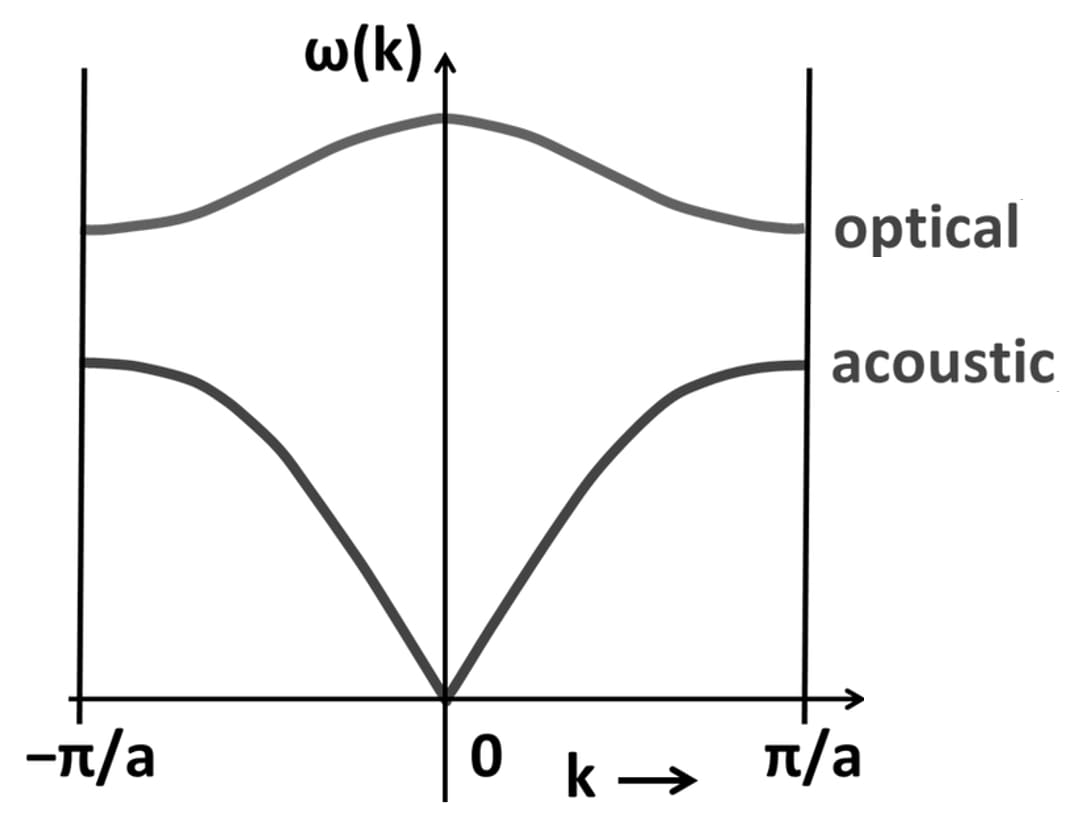
\includegraphics[width=0.4\textwidth]{Figure/Chapter 2/diatom.jpg}
\caption{\label{fig:diatom} Phonon dispersion relation for a diatomic chain.
}
\end{figure}
%These phonon frequencies and phonon polarisation vectors describe the vibrational properties of the crystal and are essential for examining phonon dispersion relations and calculating other lattice dynamical properties, such as heat capacity, thermal conductivity, and phonon density of states.

The fluctuation of phonon frequencies in respect to the wave vector $\mathbf{q}$ within the Brillouin zone is depicted by the phonon dispersion relations $\omega_{j}(\mathbf{q})$.
These connections are essential to lattice dynamics and provide a thorough understanding of the vibrational modes present within the crystal.
In crystals, the number of phonon branches corresponds to the total degrees of freedom per unit cell.
For a unit cell containing $N$ atoms, there are $3N$ branches: $3$ acoustic branches, where phonon frequencies linearly approach zero as $\mathbf{q}\rightarrow0$ and $3N-3$ optical branches, where phonon frequencies remain finite as $\mathbf{q}\rightarrow0$.
Acoustic branches are the collective, in-phase vibrations of atoms that propagate through the crystal as sound waves.  On the other hand, optical branches are the result of out-of-phase, relative motions between atoms within the unit cell and typically occur at higher frequencies.

I also provide the phonon dispersion relations of the infinite one-dimensional diatomic chain, shown in figure~\ref{fig:diatom}.

Once acquiring the phonon dispersion relations, the phonon density of states (DoS) can be computed to quantify the potential vibrational modes distributed across the range of frequencies.  This distribution is crucial for determining thermodynamic properties such as heat capacity and entropy, as well as for analysing vibrational contributions to thermal transport.
The phonon DoS \cite{Togo2015} is defined as:
\begin{equation}
\label{equ:2.11}
    \begin{split}
         g(\omega) = \frac{1}{N_{l}}\sum_{\mathbf{q}j}\;\delta(\omega-\omega_{j}(\mathbf{q})),
    \end{split}
\end{equation}
where $N_{l}$ is the number of unit cells in the lattice, and $\delta(\omega-\omega_{j}(\mathbf{q}))$ is the Dirac delta function, which ensures contributions only at the frequencies corresponding to the phonon modes.

The description of vibrational modes in the lattice, defined by acoustic and optical branches, can be improved by including quantum mechanics. This enables a quantised treatment of lattice vibrations by adding phonons as discrete energy-carrying quasiparticles. Such a framework is required for accurately collecting thermal characteristics at low temperatures and modelling phonon scattering processes that influence thermal conductivity.

In a quantum mechanical framework, the atomic displacement $u^{\alpha}_{l\kappa}$ can be treated as a quantum operator and expressed as a discrete Fourier transform of the phonon normal mode displacements, $u_{\kappa,\;j}(\mathbf{q})$ associated with the wave vector $\mathbf{q}$ and the normal mode of band index $j$: 
\begin{equation}
\label{equ:2.12}
    \begin{split}
         u^{\alpha}_{l\kappa} = \frac{1}{\sqrt{N_{l}}}\sum_{\mathbf{q}j}\;u_{\kappa,\;j}(\mathbf{q})\;\textbf{e}^{-i\mathbf{q}\cdot\mathbf{R}^{0}_{\kappa l}}\;\epsilon^{\alpha}_{\kappa,\;j}(\mathbf{q}),
    \end{split}
\end{equation}
where the summation over $j$ runs over all phonon modes.
The normal mode displacement $u_{\kappa,\;j}(\mathbf{q})$ represent the quantum-mechanical position operator and is given by:
\begin{equation}
\label{equ:2.13}
    \begin{split}
         u_{\kappa,\;j}(\mathbf{q}) = \sqrt{\frac{\hbar}{2m_{\kappa}\omega_{j}(\mathbf{q})}}\left[\hat{a}^\dagger_{j}(\mathbf{-q})+\hat{a}_{j}(\mathbf{q})\right],
    \end{split}
\end{equation}
where $\hbar$ is the reduced Planck constant, $\hat{a}^\dagger_{j}(\mathbf{-q})$ is the phonon creation operator and $\hat{a}_{j}(\mathbf{q})$ is the phonon annihilation operator.
This formulation incorporates the quantum nature of lattice vibrations, where phonon creation and annihilation operators govern the quantised energy exchange in the lattice.

Under the harmonic approximation, the lattice Hamiltonian can be expressed in terms of these operators.
Starting from the Hamiltonian in equation (\ref{equ:2.1}), the total Hamiltonian is rewritten as the sum of the kinetic energy $(\mathcal{T})$ and the harmonic potential energy $\Phi_{\text{Harm}}$:
\begin{equation}
\label{equ:2.14}
    \begin{split}
       \mathcal{H}_{\text{Harm}} &= \mathcal{T}+\Phi_{\text{Harm}}\\
       &=\sum_{\mathbf{q}j}\hbar\omega_{j}(\mathbf{q})\left[\frac{1}{2}+\hat{a}^\dagger_{j}(\mathbf{-q})\hat{a}_{j}(\mathbf{q})\right],
    \end{split}
\end{equation}
which is the Hamiltonian of quantum simple harmonic oscillation.
The second term, $\hat{a}^\dagger_{j}\hat{a}_{j}$, in equation (\ref{equ:2.14}) is the phonon number operator, which corresponds to the phonon occupation number.

From the principles of statistical mechanics, phonons, as bosonic quasiparticles, obey the Bose-Einstein distribution, as their occupation number quantifies the thermal population of each vibrational mode in equilibrium.
The phonon occupation number can, therefore, be expressed as:
\begin{equation}
\label{equ:2.15}
       n_{j}(\mathbf{q}) = \frac{1}{\mathbf{e}^{\left(\hbar\omega_{j}(\mathbf{q})/k_{\text{B}}T\right)}-1},
\end{equation}
where $n_{j}(\mathbf{q})$ gives the average number of phonons in mode $j$ at wave vector $\mathbf{q}$, $k_{\text{B}}$ is the Boltzmann constant, and $T$ is the temperature.
In the canonical ensemble system, the Hamiltonian in equation (\ref{equ:2.14}) can be solved to obtain the energy of phonons as:
\begin{equation}
\label{equ:2.16}
    \begin{split}
       E_{\text{Harm}} &= \sum_{\mathbf{q}j}\hbar\omega_{j}(\mathbf{q})\left(\frac{1}{2}+n_{j}(\mathbf{q})\right).
    \end{split}
\end{equation}
%Using thermodynamic relations, this phonon energy can be used to calculate thermal properties as a function of temperature, such as Helmholtz free energy $F$, entropy $S$ and the isochoric (constant-volume) heat capacity $C_{V}$ \cite{dove_2005}.
This phonon energy can be used to calculate the isochoric heat capacity $C_{V}$, which is essential to our research since it serves as a foundation for calculating lattice thermal conductivity \cite{Togo2015}.
By employing the thermodynamic relation of the heat capacity \cite{dove_2005},
we, therefore, obtain 
\begin{equation}
\label{equ:2.17}
    \begin{split} 
   C_{V}(T)  & = \left( \frac{\partial E_{\text{Harm}}(T)}{\partial T} \right)_V\\
       &= \sum_{\mathbf{q}j}\;C_{V,\;j}(\mathbf{q},\;T)\\
       &=\sum_{\mathbf{q}j}k_{\text{B}}\left(\frac{\hbar\omega_{j}(\mathbf{q})}{k_{\text{B}}T}\right)^{2}\frac{\mathbf{e}^{\left(\hbar\omega_{j}(\mathbf{q})/k_{\text{B}}T\right)}}{\left[ \mathbf{e}^{\left(\hbar\omega_{j}(\mathbf{q})/k_{\text{B}}T\right)}-1 \right]^{2}}.
    \end{split}
\end{equation}
This equation describes how phonons contribute to the heat capacity of the system, with contributions from all phonon modes indexed by $\mathbf{q}$ and $j$.\footnote{In addition to phonons, electrons also contribute to the heat capacity, particularly in metals. This electronic contribution is typically linear in temperature at low \( T \), but is negligible in insulators and semiconductors where electronic excitations are thermally suppressed. \cite{ashcroft_mermin}}

%not sure how to realate with electron
\paragraph{}
Here, we can see the harmonic approximation simplifies the lattice potential by preserving solely quadratic (second-order) terms in atomic displacements.  Consequently, atomic vibrations can be represented as a collection of isolated, non-interacting phonon modes with constant frequencies that remain unaffected by temperature variations.
In this context, temperature-dependent thermal parameters, including isochoric heat capacity, can be precisely computed utilising Bose-Einstein statistics for phonon occupancy. 
However, the lattice thermal conductivity cannot be computed realistically under this approximation: because phonon-phonon interactions are absent, no intrinsic phonon scattering occurs, and the thermal conductivity formally diverges and becomes infinite. 
To model thermal resistance and predict finite conductivity, one must include cubic (third-order) anharmonic terms, which give rise to three-phonon scattering processes.
%Under the harmonic approximation, thermal properties \cite{dove_2005} can be calculated as functions of temperature.
%However, the lattice thermal conductivity is infinite within this approximation because phonon-phonon scattering, which requires cubic anharmonicity, is neglected.

The cubic anharmonic crystal potential, which introduces phonon-phonon interactions, can be expressed as a sum of three-phonon collisions:
\begin{equation}
\label{equ:2.18}
\begin{split}
\Phi_{\text{Anh}} &= \sum_{j_{1},j_{2},j_{3}} \sum_{\mathbf{q}_{1},\mathbf{q}_{2},\mathbf{q}_{3}} \Phi_{j_{1},j_{2},j_{3}}(\mathbf{q}_{1}, \mathbf{q}_{2}, \mathbf{q}_{3}) \\
&\quad \times \left(\hat{a}^\dagger_{j_{1}}(-\mathbf{q}_{1}) + \hat{a}_{j_{1}}(\mathbf{q}_{1})\right)\\
&\quad \times \left(\hat{a}^\dagger_{j_{2}}(-\mathbf{q}_{2}) + \hat{a}_{j_{2}}(\mathbf{q}_{2})\right)\\
&\quad \times \left(\hat{a}^\dagger_{j_{3}}(-\mathbf{q}_{3}) + \hat{a}_{j_{3}}(\mathbf{q}_{3}) \right),
\end{split}
\end{equation}
where $\Phi_{j_{1},j_{2},j_{3}}(\mathbf{q}_{1}, \mathbf{q}_{2}, \mathbf{q}_{3})$ denotes the strength of interaction among the three phonons with wave vector
$(\mathbf{q}_{1}, \mathbf{q}_{2}, \mathbf{q}_{3})$ in the normal mode $(j_{1},j_{2},j_{3})$.
The explicit form of this interaction strength can be expressed through a discrete Fourier transform of the cubic anharmonic force constant in Cartesian coordinates, $\Phi^{(3)}_{\alpha l_{1}\kappa_{1},\;\beta l_{2}\kappa_{2},\;\gamma l_{3}\kappa_{3}}$,  as:
\begin{equation}
\label{equ:2.19}
\begin{split}
\Phi_{j_{1},j_{2},j_{3}}(\mathbf{q}_{1}, \mathbf{q}_{2}, \mathbf{q}_{3}) &= \frac{1}{6\sqrt{N_{l}}} \sum_{\alpha\beta\gamma} \sum_{\kappa_{1}\kappa_{2}\kappa_{3}}\;\epsilon^{\alpha}_{\kappa_{1},\;j_{1}}(\mathbf{q}_{1})\;\epsilon^{\beta}_{\kappa_{2},\;j_{2}}(\mathbf{q}_{2}) \;\epsilon^{\gamma}_{\kappa_{3},\;j_{3}}(\mathbf{q}_{3}) \\
&\quad \times \sqrt{\frac{\hbar}{2m_{\kappa_{1}} \omega_{j_{1}}(\mathbf{q}_{1})}} 
\sqrt{\frac{\hbar}{2m_{\kappa_{2}} \omega_{j_{2}}(\mathbf{q}_{2})}} 
\sqrt{\frac{\hbar}{2m_{\kappa_{3}} \omega_{j_{3}}(\mathbf{q}_{3})}} \\
&\quad \times \sum_{l_{1}, l_{2}, l_{3}} \Phi^{(3)}_{\alpha l_{1}\kappa_{1},\;\beta l_{2}\kappa_{2},\;\gamma l_{3}\kappa_{3}}\cdot \:\textbf{e}^{i\mathbf{q}_{2}\cdot\left(\mathbf{R}^{0}_{l_{2}\kappa_{2}}-\mathbf{R}^{0}_{l_{1}\kappa_{1}}\right)}\\
&\quad \cdot \:\textbf{e}^{i\mathbf{q}_{3}\cdot\left(\mathbf{R}^{0}_{l_{3}\kappa_{3}}-\mathbf{R}^{0}_{l_{1}\kappa_{1}}\right)} \cdot \:\textbf{e}^{i\left(\mathbf{q}_{1} + \mathbf{q}_{2} + \mathbf{q}_{3}\right)\cdot\mathbf{R}^{0}_{l_{1}\kappa_{1}}}\\
&\quad \times \delta^{\ast}(\mathbf{q}_{1} + \mathbf{q}_{2} + \mathbf{q}_{3}),
\end{split}
\end{equation}
where $\delta^{\ast}(\mathbf{q}_{1} + \mathbf{q}_{2} + \mathbf{q}_{3})$ enforces momentum conservation and is defined as:
\begin{equation}
\label{equ:2.20}
\delta^{\ast}(\mathbf{q}_{1} + \mathbf{q}_{2} + \mathbf{q}_{3}) =
\begin{cases} 
1, & \text{if } \mathbf{q}_{1} + \mathbf{q}_{2} + \mathbf{q}_{3} \text{ is a reciprocal lattice vector}, \\
0, & \text{otherwise}.
\end{cases}
\end{equation}
Many-body perturbation theory (MBPT)\footnote{Many-body perturbation theory (MBPT) provides highly accurate calculations of phonon anharmonicity in crystalline materials with weak anharmonic interactions. However, for materials exhibiting strong anharmonicity, such as perovskites, thermoelectric materials, and superconducting hydrides, alternative methods like first-order self-consistent phonon theory are often more suitable \cite{Tadano2018}.} 
can be used to extract the anharmonic self-energy of phonons.
The phonon self-energy is generally a complex function comprising a real part, $\Delta(\omega)$, and the imaginary part $\Gamma(\omega)$ corresponding to a phonon of frequency $\omega$ \cite{R.A.Cowley}.
The real part, $\Delta(\omega)$, is associated with the phonon frequency renormalisation. The imaginary part, $\Gamma(\omega)$, represents an energy loss term associated with phonon scattering processes and is inversely related to the phonon lifetime.

To calculate the realistically consistent thermal conductivity of a crystal necessitates consideration of the imaginary component, which, within the context of second-order perturbation theory, is expressed as:
%To establish a connection with the thermal conductivity of a crystal, we focus on the imaginary part which, within the framework of second-order perturbation theory, is given by:
\begin{equation}
\label{equ:2.21}
    \begin{split}
        \Gamma_{j}(\omega;\;\mathbf{q}) = \frac{18\pi}{\hbar^{2}}\sum_{j_{2},j_{3}} \sum_{\mathbf{q}_{2},\mathbf{q}_{3}}&\left|\Phi_{j,j_{2},j_{3}}(-\mathbf{q}, \mathbf{q}_{2}, \mathbf{q}_{3}) \right|^{2}\\
        &\bigg[\left(n_{j_{2}}(\mathbf{q}_{2})+n_{j_{3}}(\mathbf{q}_{3})+1\right)\cdot\delta\left(\omega-\omega_{j_{2}}(\mathbf{q}_{2})-\omega_{j_{3}}(\mathbf{q}_{3})\right)\\
        &+\left(n_{j_{2}}(\mathbf{q}_{2})-n_{j_{3}}(\mathbf{q}_{3})\right)\cdot\delta\left(\omega-\omega_{j_{2}}(\mathbf{q}_{2})\right)\\
        &-\left(n_{j_{2}}(\mathbf{q}_{2})-n_{j_{3}}(\mathbf{q}_{3})\right)\cdot\delta\left(\omega-\omega_{j_{2}}(\mathbf{q}_{2})-\omega_{j_{3}}(\mathbf{q}_{3})\right)\bigg]
    \end{split}
\end{equation}
where $n_{j}(\mathbf{q})$ is the phonon occupation number defined in Eq.~\eqref{equ:2.15}.
$2\Gamma_{j}(\omega;\;\mathbf{q})$ represents the phonon line-width for the phonon mode $(\mathbf{q},\;j)$.
By taking the inverse of the phonon line-width, the corresponding phonon lifetime can be determined,
\begin{equation}
\label{equ:2.22}
       \tau_{j}(\mathbf{q}) = \frac{1}{2\Gamma_{j}(\omega;\;\mathbf{q})}.
\end{equation}

%From the linearised phonon Boltzmann transport equation (LBTE) under the single-mode relaxation-time (SMRT) approximation \cite{srivastava_1990}, 

%the lattice thermal conductivity \( \kappa \) can be computed by combining the mode-resolved specific heat capacity (Equation~\ref{equ:2.17}) and the phonon lifetime (Equation~\ref{equ:2.22}). 

%In the SMRT approximation, the phonon lifetime \( \tau_j(\mathbf{q}) \) is assumed to be equivalent to the single-mode relaxation time \( \tau_j(\mathbf{q})^{\text{SMRT}} \), where each phonon mode relaxes independently of all others. 
%This simplification enables efficient computation of \( \kappa \), but neglects mode-coupling effects that may be significant in strongly anharmonic systems.
From the linearised phonon Boltzmann transport equation (LBTE) under the single-mode relaxation-time (SMRT) approximation \cite{srivastava_1990}, the phonon lifetime \( \tau_j(\mathbf{q}) \) is approximated to be the single-mode relaxation time \( \tau_j(\mathbf{q})^{\text{SMRT}} \).
This approximation assumes that each phonon mode relaxes independently of all others, simplifying the complex interactions in the phonon system. This allows us to efficiently calculate the thermal conductivity by neglecting mode-coupling effects that may be substantial in strongly anharmonic systems.
Thus combining the mode-resolved specific heat capacity (Equation~\eqref{equ:2.17}) and the phonon lifetime (Equation~\eqref{equ:2.22}), the lattice thermal conductivity is expressed as
\begin{equation}
\label{equ:2.23}
       \kappa = \frac{1}{N_{l}\cdot \Omega_{\text{cell}}}\sum_{\mathbf{q}j}\Big[\mathbf{v}_{j}(\mathbf{q})\otimes \mathbf{v}_{j}(\mathbf{q})\Big]\cdot C_{V,\;j}(\mathbf{q},\;T)\cdot \tau_{j}(\mathbf{q})^{\text{SMRT}},
\end{equation}
where $\Omega_{\text{cell}}$ is the volume of each unit cell, and $N_{l}$ denotes the total number of atoms per a unit cell.
The phonon group velocities $\mathbf{v}_{j}(\mathbf{q})$ can be given by the slope of the phonon dispersion relation,
\begin{equation}
\label{equ:2.24}
   \mathbf{v}_{j}(\mathbf{q})=\frac{\partial \omega_{j}(\mathbf{q})}{\partial \mathbf{q}}.
\end{equation}
Alternatively, the components of the group velocity, $v^{\alpha}_{j}(\mathbf{q})$, can be directly calculated by differentiating the eigenvalue in Equation~\eqref{equ:2.9} with respect to the phonon wave vector \cite{Togo2015-qf}:
\begin{equation}
\label{equ:2.25}
        v^{\alpha}_{j}(\mathbf{q}) = \frac{1}{2\omega_{j}(\mathbf{q})}\sum_{\kappa\beta}\sum_{\kappa'\gamma}\;\epsilon^{\beta}_{\kappa,\;j}(\mathbf{q})
        \;\frac{\partial D_{\beta\gamma,\;\kappa\kappa'}(\mathbf{q})}{\partial q_{\alpha}}\;\epsilon^{\gamma}_{\kappa',\;j}(\mathbf{q}).
\end{equation}
%These expressions are essential for understanding the functionalities and computational protocols implemented in tools such as \textsc{phonopy} and \textsc{phono3py}, which are widely used for phonon and thermal transport calculations.
I have discussed the fundamental relations as used in \textsc{phonopy} and \textsc{phono3py}, which form the basis for understanding the functionalities and computational procedures underlying these widely used tools for phonon and thermal transport calculations. 

While the force-constant approach described above is the most widely used route to obtain phonon spectra from first principles, phonons can also be computed from finite-temperature molecular dynamics simulations. 
In such cases, we can extract vibrational information by analysing the velocity autocorrelation function or the dynamical structure factor obtained from a sufficiently long MD trajectory (classical or \textit{ab initio} MD). 
These time-correlation methods yield phonon densities of states and, when combined with appropriate projections, phonon dispersions, providing an alternative to the direct finite-difference or density-functional perturbation theory approaches.


\section{Density Functional Theory} \label{sec:2.2}
\paragraph{}
Harmonic and cubic anharmonic force constants are the key parameters which describe the phonon properties of materials.
The calculation of these force constants via the finite difference method requires a set of forces acting on atoms in the system.
One way to calculate these forces is by using electronic structure calculations, such as Density Functional Theory (DFT).

Density Functional Theory (DFT) is a powerful computational method widely used in quantum chemistry and condensed matter physics to study the electronic structure of atoms, molecules, and solids.
By approximating the many-body Schrödinger equation with an $O(N^{3})$-based method, DFT offers a computationally efficient framework to investigate fundamental properties such as electronic energies, molecular geometries, and spectroscopic features.
This chapter provides a detailed explanation of the theoretical foundations and computational methodologies associated with~DFT.

\subsection{Theoretical Foundations}  \label{sec:2.2.1}
%$The starting point of quantum mechanical calculations is the time-independent Schr\"{o}dinger equation for a system of interacting electrons: where is the Hamiltonian, is the many-body wavefunction, and is the total energy.
The first point of quantum mechanical calculations is the time-independent Schr\"{o}dinger equation for a system of interacting electrons,
\[
    \hat{H} \Psi = E \Psi,
\]
where $\hat{H}$ is the Hamiltonian operator, $\Psi$ is the many-body wavefunction, and $E$ is the total energy of the system.
The Hamiltonian includes the kinetic energy of the electrons, the electron-nucleus attraction, and the electron-electron Coulomb repulsion.
Solving this equation directly is computationally infeasible for systems with many electrons due to the exponential growth of the wavefunction's complexity $O(N!)$.

Establishing the Hohenberg-Kohn (H-K) theorems is a key step in the development of density functional theory (DFT).
These theorems prove that the ground-state energy of a many-electron system is uniquely determined by its electron density. 
Furthermore, the ground-state electron density minimises a total energy functional of the electron density, which includes contributions from the kinetic energy, the external potential, the Hartree energy, and the exchange-correlation energy.

Building on this H-K foundation, the Kohn-Sham (KS) approach simplifies the many-electron problem by introducing a system of non-interacting electrons that reproduces the ground-state electron density of the interacting system.
The KS equations, which govern this non-interacting system, are expressed as:
\begin{equation}
\label{equ:2.26}
\left(-\frac{\hbar^2}{2m} \nabla^2 + V_{\text{eff}}(\mathbf{r})\right) \psi_i(\mathbf{r}) = \epsilon_i \psi_i(\mathbf{r}),
\end{equation}
where $\psi_i(\mathbf{r})$ are the Kohn–Sham orbitals, $\epsilon_i$ are their associated eigenvalues, and $V_{\text{eff}}(\mathbf{r})$ is the effective potential, given by:
\begin{equation}
\label{equ:2.27}
V_{\text{eff}}(\mathbf{r}) = V_{\text{ext}}(\mathbf{r}) + V_{\text{Hartree}}(\mathbf{r}) + V_{\text{xc}}(\mathbf{r}),
\end{equation}
with $V_{\text{ext}}(\mathbf{r})$, $V_{\text{Hartree}}(\mathbf{r})$, and $V_{\text{xc}}(\mathbf{r})$ representing the known external, exact Hartree, and approximate exchange–correlation potentials, respectively.

In typical condensed-phase systems the external potential $V_{\text{ext}}(\mathbf{r})$ due to the nuclei dominates, as it contains the strong Coulomb attraction at each nuclear site. 
The Hartree term $V_{\text{Hartree}}(\mathbf{r})$ represents the classical electrostatic repulsion of the electron density.
It is generally an order of magnitude smaller but still comparable to $V_{\text{ext}}$ in regions of high electron density. 
The exchange–correlation potential $V_{\text{xc}}(\mathbf{r})$ is the smallest component.
Although crucial for accuracy, it typically contributes only a few to tens of percent of the total effective potential depending on the material and the functional used. 
These relative magnitudes motivate why $V_{\text{ext}}$ sets the overall scale of the problem, while $V_{\text{Hartree}}$ and $V_{\text{xc}}$ provide successively finer corrections to the electronic structure.

\subsection{Computational methodologies} \label{sec:2.2.2}
The first step in a DFT calculation is to define the atomic positions and the system geometry.
For molecular systems, atomic arrangements are specified using Cartesian or internal coordinates.
For solid-state systems, additional lattice parameters and unit cell configurations are required to define the periodic structure of the material.
 
The electronic wavefunctions in a DFT calculation are typically represented using a finite basis set, which is chosen based on the nature of the system being studied.
Common types of basis sets include:
\begin{itemize}
    \item[1] \textbf{Gaussian-Type Orbitals (GTOs)}:  Frequently employed in molecular systems because of their computational efficacy in depicting localised wavefunctions.  However, GTO basis sets sometimes exhibit overcompleteness, affecting the extrapolation to the complete (basis-free) limit.
    \textbf{Plane Waves (PW)}:  Commonly used in periodic systems, as they effectively reflect delocalised electronic states in crystals.  Although plane waves may be inefficient for systems with high ionic density due to the requirement for a substantial energy cutoff, their intrinsic orthogonality allows systematic convergence to the complete basis set limit.
\end{itemize}


The choice of basis set significantly impacts the computational cost and accuracy of the calculation, making it an important consideration during problem setup.

The accuracy of a DFT calculation is also strongly influenced by the selection of the exchange-correlation (XC) functional, which approximates the many-body effects of electron exchange and correlation. Common categories of XC functionals are
\begin{itemize}
    \item[1] \textbf{Local Density Approximation (LDA):} Relies solely on the local electron density, parametrised using quantum Monte Carlo results for the homogeneous electron gas (HEG), and is most accurate for systems with slowly varying electron density, such as metals.
    \item[2] \textbf{Generalised Gradient Approximation (GGA):} Improves upon LDA by incorporating the gradient of the electron density, allowing for greater accuracy in systems with sharply varying electron densities, such as insulates and semiconductor. Popular examples include the Perdew-Burke-Ernzerhof (PBE) functional.
    \item[3] \textbf{Meta-GGA Functionals:} Represent the next rung on “Jacob’s ladder” of DFT approximations by including, in addition to the density and its gradient, information about the kinetic-energy density or the Laplacian of the density. Examples include SCAN (Strongly Constrained and Appropriately Normed) \cite{Sun2015} and TPSS (Tao–Perdew–Staroverov–Scuseria) \cite{Tao2003} functionals. These functionals can improve predictions of structural and thermochemical properties compared with standard GGAs, although the improvement is not universal.
    \item[4] \textbf{Hybrid Functionals:} Combine DFT correlation with a fraction of exact Hartree–Fock exchange, providing a more accurate treatment of electron interactions for many systems. Examples include B3LYP, widely used in molecular chemistry, and HSE06, commonly applied in solid-state calculations. 
\end{itemize}

Climbing Jacob's ladder \cite{Tao2003} often increases the formal sophistication of the functionality and often enhances accuracy for specific system categories; but, it does not ensure consistently superior outcomes.  
For example, a well-parameterised GGA can outperform a meta-GGA for specific properties, and hybrids can sometimes degrade predictions for metals even though they improve molecular energetics. 
Thus, the choice of functional should be made on a property- and system-specific basis, taking into account both accuracy requirements and computational cost.

After selecting the exchange-correlation (XC) functional, the Kohn-Sham equations are solved using the self-consistent field (SCF) procedure, an iterative algorithm designed to achieve convergence of both the electron density and the total energy.
The SCF procedure involves the following steps:
\begin{itemize}
    \item[1] Initial Guess: An initial guess for the electron density is generated, which may be based on atomic orbitals, a uniform density, or results from previous calculations.
    \item[2] Potential Update: the current electron density is used to calculate the effective potential. This potential includes contributions from the external potential, Hartree potential, and exchange-correlation potential.
    \item[3] Solve Kohn-Sham Equations: The Kohn-Sham equations are solved to obtain the updated Kohn-Sham orbitals $(\psi_i)$ and their associated eigenvalues $(\epsilon_i)$.
    \item[4] Convergence Check: The updated electron density and total energy are compared to the values from the previous iteration. If the changes are below predefined thresholds, the calculation is considered converged. Otherwise, the process is repeated using the updated density. 
\end{itemize}

The SCF procedure ensures the self-consistency of the electronic structure, which is essential for achieving accurate and reliable results in DFT calculations. It is essential to obtain well-converged energy and forces from DFT calculations for our research, as we seek to predict machine-learned force constants based on this reference data.  We give the SCF convergence parameters in the techniques part of Chapter~\ref{ch:3} to furnish an appropriate dataset for training.
%The SCF procedure ensures the self-consistency of the electronic structure, which is essential for achieving accurate and reliable results in DFT calculations.
%The accuracy and transferability of machine-learned force constants critically depend on the quality of the reference data; therefore, ensuring well-converged energies and forces from DFT calculations is essential. The convergence settings used to generate training data for machine learning models will be discussed in the methodology section of Chapter~\ref{ch:3}.
%The specific settings for the convergence criteria, used to compute the energies and forces required for phonon calculations, will be detailed in the methodology section of Chapter \ref{ch:3}.
\cite{Sun2015}
Although DFT provides a precise framework for calculating electronic structures and associated properties, its computational expense becomes excessive for large systems or when extensive configuration space sampling is required, such as in the generation of training data for machine learning models.  To come across this limitation, machine learning, particularly Gaussian processes (GPs), has emerged as an efficient surrogate model, as an approximate model, for predicting energy, forces, and related observables with significantly reduced computational costs.  In the subsequent section, we outline the fundamental notions underpinning Gaussian process regression.

\newpage
\section{Gaussian Processes} \label{sec:2.3}
\paragraph{}
We present the mathematical foundations of the conventional Gaussian process (GP) model and its derivative model in this section on GPs.
After that, a survey of relevant research will be given, emphasising its uses and importance in the domains of computational chemistry and physics.

\subsection{Conventional Model} \label{sec:2.3.1}
The concept of a (multivariate) Gaussian distribution can be extended using a \textit{Bayesian} framework, leading to the formulation of a Gaussian process (GP) model \cite{RasmussenW06}.
Mathematically, Gaussian processes are defined as a collection of random variables, any finite subset of which follows a (multivariate) Gaussian distribution.
A random vector (descriptor), $\mathbf{x}$, can be indexed by time, space, or other inputs; this set of descriptors constitutes the \textbf{input space}.
In our case, the input space corresponds to Atomic Cluster Expansion descriptors of a given configuration, while the \textbf{target values} are the physical quantities to be predicted (such as energies, forces).

A GP is fully characterised by its mean function and covariance function.
These functions are defined for a real function $f(\mathbf{x})$ as:
\begin{equation}
    \label{equ:2.28}
    \begin{split}
     m(\mathbf{x}) &= \mathbb{E}[f(\mathbf{x})],\\
     k(\mathbf{x},\;\mathbf{x}^{*}) &=\mathbf{Cov}\left(f(\mathbf{x}), f(\mathbf{x}^{*})\right)\\
     &= \mathbb{E}[(f(\mathbf{x}) - m(\mathbf{x}))(f(\mathbf{x}^{*}) - m(\mathbf{x}^{*}))],
    \end{split}
\end{equation}
where $m(\mathbf{x})$ represents the expected value (mean) of the function at descriptor $\mathbf{x}$, and $k(\mathbf{x},\;\mathbf{x}^{*})$ defines the covariance between the function evaluated at $\mathbf{x}$ and $\mathbf{x}^{*}$.
The Gaussian process, fully defined by its mean function and covariance function, can be interpreted as a \textbf{prior distribution} over the space of possible functions,
\begin{equation}
    \label{equ:2.29}
    f(\mathbf{x}) \sim \mathcal{GP} \left( m(\mathbf{x}), k(\mathbf{x},\; \mathbf{x}^{*}) \right),
\end{equation}
where $m(\mathbf{x})$ and $k(\mathbf{x},\;\mathbf{x}^{*})$ are defined in equation ~\eqref{equ:2.28}, describing the relationship between function values at different points in the input space.
This means that before seeing any data we have a prior belief about the function’s behaviour (encoded by $m$ and $k$). 
Given observed data $\mathcal{D}=\{\mathbf{x}_i,y_i\}$, Bayes’ theorem updates this belief to a \textbf{posterior distribution}:
\begin{equation}
\label{equ:bayes}
p(f\,|\,\mathcal{D}) = \frac{p(\mathcal{D}\,|\,f)\,p(f)}{p(\mathcal{D})},
\end{equation}
where:
\begin{itemize}
  \item $p(f)$ is the \textbf{prior}, our assumption about the function before seeing the data (here, the GP defined by $m$ and $k$);
  \item $p(\mathcal{D}\,|\,f)$ is the \textbf{likelihood}, which measures how probable the observed targets are for a given function;
  \item $p(f\,|\,\mathcal{D})$ is the \textbf{posterior}, our updated belief about the function after observing the data.
\end{itemize}
Because GPs maintain full probability distributions over functions and explicitly update them via Bayes’ theorem, they are referred to as \textbf{Bayesian} models.
%(Note that “prior dataset” is a misnomer: we have a dataset, and separately we have a prior distribution that expresses assumptions before any data are incorporated.)

The mean function is often assumed to be zero, i.e. $m(\textbf{x}) = 0$, simplifying in many Gaussian process applications.
The covariance function $k(\textbf{x},\:\textbf{x}^{*})$ is commonly referred to as the GP "\textit{kernel}".
This \textit{kernel} is a pairwise function defined on two $d$-dimensional descriptors, $\mathbf{x}$ and $\mathbf{x}^{*}$, and specifies the correlation between the function values at these points.
In essence, it maps two $d$-dimensional vectors to a single scalar value, 
\[k(\cdot,\:\cdot):\mathbb{R}^{d}\times\mathbb{R}^{d}\rightarrow\mathbb{R},\]
The simplest kernel used in a GP model is the \textit{dot-product} (or \textit{linear}) kernel, which is defined as:

\begin{equation} \label{equ:2.30}
k(\mathbf{x},\;\mathbf{x}^{\ast}) = \mathbf{x} \cdot \mathbf{x}^{\ast}. 
\end{equation}
This kernel reduces Gaussian process regression to linear regression. A more generalized version of the \textit{linear} kernel is the \textit{polynomial} kernel, expressed as:
\begin{equation} \label{equ:2.31}
    k(\mathbf{x},\;\mathbf{x}^{\ast}) = (\mathbf{x} \cdot \mathbf{x}^{\ast})^{\zeta}.
\end{equation}
where $\zeta$ represents the degree of the polynomial.
In addition to these, various other kernels have been developed, including the \textit{Mat\'{e}rn32}, \textit{Mat\'{e}rn52}, and \textit{periodic} kernels.
Detailed definitions of these kernels can be found in Rasmussen's book \cite{RasmussenW06}.

In addition to the linear and polynomial kernels, one of the most widely used kernels in Gaussian process models is the \textit{squared exponential} kernel, also known as the \textit{radial basis function (RBF)} or simply the \textit{Gaussian} kernel, defined as:
\begin{equation} \label{equ:2.32}
        \begin{split}
            k(\mathbf{x},\;\mathbf{x}^{*})= \mathbf{exp}\left[-\frac{1}{2}d(\mathbf{x},\;\mathbf{x}^{*})^{2}\right],
        \end{split}
\end{equation}
where $d(\mathbf{x},\;\mathbf{x}^{*})=\lVert\mathbf{x}-\mathbf{x}^{*}\rVert_{2}$ is the Euclidean metric.

This kernel is stationary and isotropic, depending only on the distance between points, and is infinitely differentiable, implying a very strong prior preference for smooth.
These properties make the RBF kernel a default choice for modelling smooth physical processes. 
However, it can perform poorly for rough or discontinuous data-generating functions, or for nonstationary behaviour where the characteristic lengthscale varies across the input space; in such cases kernels with weaker smoothness assumptions (e.g.\ Matérn) or locally adaptive/composite kernels may be more appropriate.

Building on the concept of Gaussian processes (GPs) discussed above, we now explore how this framework can be applied in surrogate modelling physics, such as regression tasks.
A common application of GP models in this domain is the analysis and prediction of potential energy surfaces (PESs). 
Specifically, the goal of a GP model in such cases is to predict the continuous PES $E^{*}(\mathbf{x}^{*})$, given the input $\mathbf{x}^{*}$, discrete training datapoints $\mathbf{x}$ and the corresponding PES $E(\mathbf{x})$.

To build a GP model, we need to construct the joint Gaussian distribution between those two datapoints with an $2$-dimensional zero-mean vector, as:
%By definition of building a GP model, the joint Gaussian distribution between those two data is required to be constructed, with an $2$-dimensional zero-mean vector, as:
\begin{equation}
    \label{equ:2.33}
         \begin{bmatrix}
         E\\
         E^{*}\\
         \end{bmatrix}
        \;\mathtt{\sim}\;
        \mathcal{GP}_{2}\left(
        \begin{bmatrix}
         0\\
         0\\
         \end{bmatrix}\:
         ;\:\begin{bmatrix}
             k(\mathbf{x},\:\mathbf{x})+\sigma^{2} & k(\mathbf{x},\:\mathbf{x}^{*})\\
             k(\mathbf{x}^{*},\:\mathbf{x}) & k(\mathbf{x}^{*},\:\mathbf{x}^{*})\\
         \end{bmatrix}\right),
\end{equation}  
where $\sigma^{2}$ is the observation noise associated with the PES $E(\mathbf{x})$.

This noise arises from electronic structure calculations and can be expressed as \[\tilde{E}(\mathbf{x})=E(\mathbf{x})+ \epsilon,\] where the uncertainty $\epsilon\in\mathbb{R}$ can be presumed to be normal distributed with a mean of zero and a variance of $\sigma^{2}$.
This is defined as:
\begin{equation}
    \label{equ:2.34}
        \epsilon\\
        \;\mathtt{\sim}\;
        \mathcal{N}\left(0\:
         ;\; \sigma^{2}\\
             \right).
\end{equation}
Therefore, the posterior prediction for $E^{*}$ is given by
\begin{equation}
    \label{equ:2.35}
        E^{*}|\;\mathbf{x}^{*},\;\mathbf{x},\;E\\
        \;\mathtt{\sim}\;
        \mathcal{GP}\left(
        m^{\star}(\mathbf{x}^{*},\;\mathbf{x},\;E)\:
         ;\; k^{\star}(\mathbf{x},\:\mathbf{x}^{*})\\
             \right),
\end{equation}
where $m^{\star}$ represents the posterior mean expressed as,
\begin{equation}
    \label{equ:2.36}
        m^{\star}(\mathbf{x},\;\mathbf{x}^{*},\;E)\:\\
         = \; k(\mathbf{x},\:\mathbf{x}^{*})\cdot\left(k(\mathbf{x},\:\mathbf{x})+\sigma^{2}\right)^{-1}\cdot E,
\end{equation}
and $k^{\star}$ is the corresponding posterior covariance derived from
\begin{equation}
    \label{equ:2.37}
        k^{\star}(\mathbf{x},\;\mathbf{x}^{*},\;E)\:\\
         = \; k(\mathbf{x}^{*},\:\mathbf{x}^{*}) + k(\mathbf{x},\:\mathbf{x}^{*})\cdot\left(k(\mathbf{x},\:\mathbf{x})+\sigma^{2}\right)^{-1}\cdot k(\mathbf{x}^{*},\:\mathbf{x}).
\end{equation}
In physics, Gaussian processes (GPs) have been used extensively. As previously mentioned, GPs can be used for modelling the electronic potential energy surfaces (PESs) of \(N\)-atomic systems with the help of previous information.
Typically, density functional theory (DFT) computations provide potential energies and atomic forces at specific input structures, which form the training data for the GP.

Each structure and its associated potential energy can be represented for GP modelling as a scalar target \(E_{i}\) and a \(3N\)-dimensional Cartesian descriptor \(\mathbf{x}_{i}\), respectively.
A total of \(n\) structures can then be arranged into a \(3N \times n\) descriptor matrix \(\mathbf{X}\) and an \(n\)-dimensional target vector \(\mathbf{E}\), yielding a \textit{training} or \textit{test} dataset compatible with GP models.

For \(N\) datapoints, exact GPs require inversion of an \(N\times N\) covariance matrix when training, which scales as \(\mathcal{O}(N^3)\) in time and \(\mathcal{O}(N^2)\) in memory. 
Predictions at \(N^\ast\) new structures scale as \(\mathcal{O}(N\,N^\ast)\)–\(\mathcal{O}(N^2\,N^\ast)\) depending on whether predictive variances are computed. 
This cubic cost limits the practical application of exact GPs to only a few tens of thousands of training points. 
Sparse or approximate GP methods alleviate this bottleneck by introducing a much smaller set of \(M\ll N\) inducing points; training then scales as \(\mathcal{O}(n\,M^2)\) and prediction as \(\mathcal{O}(M\,N^\ast)\), making GPs tractable for much larger datasets at the expense of an approximation whose quality depends on how well the inducing points capture the underlying data structure.

Beyond computational cost, another key challenge for GP models of materials is ensuring size transferability. 
Total energy is an extensive quantity, so to apply a GP model across system sizes different from those used in training it must be reformulated as an additive or local model in which an intensive latent function of each atom’s environment is learned and the total energy is expressed as the sum of these contributions.
%; this approach, common in ACE/SOAP-based GPs, gives true size transferability, whereas simply training on E/N does not because the kernel and representation remain global. 
In our work we use the global Gaussian process approach, which represents each configuration by a single whole-system descriptor and applies a global kernel. Within this framework, the energy prediction cannot be made intensive and size-transferable without restructuring the model. This global choice has the advantage of capturing collective, long-range correlations and being conceptually simple for fixed-size systems, but at the cost of losing principled size transfer and data efficiency when locality holds.

\subsection{Reviews on Gaussian Processes for Molecules and Materials}
Bart\'{o}k's and Szlachta's PhD thesis \cite{thesis1, thesis2} were the first to propose this study of electronic PESs using a GP technique in 2010 and 2013. 
Simple systems with a few degrees of freedom, such as polarised water \cite{Handley2009}, a crystalline silicon \cite{Bartk2018, Strickson2019}, \ch{N4} \cite{Cui2016}, methyl chloride \cite{Dral2017}, or a molecule like \ch{H3O+} \cite{Dai2020}, were effectively treated using a GP approach.
However, because the GP kernel computation does not scale well, examining a more complicated structures with higher DoFs results in a costly GP calculation.

Several optimisation strategies can be used to lower the computing cost of GP. 
For instance \cite{RasmussenW06}, a GP kernel matrix was reduced in size using a sparse approach, which involves converting it into a smaller kernel matrix with a low rank approximation.%all zero components eliminated.
For the protonated imidazole dimer (\ch{C6N9N4+}), Sugisawa et al. successfully implemented this sparse GP to the $51$-dimensional PES \cite{Sugisawa2020}.

A composite GP kernel, which is created by adding or multiplying two or more distinct kernels, is an additional method to increase the complexity of the GP model.
By raising the GP model complexity, the number of data points needed for a given accuracy is decreased while the GP model becomes more complex.
Global PESs of \ch{H3O+} were interpolated and extrapolated using this method by J. Dai and R. V. Krems \cite{Dai2020}.

Furthermore, by differentiating a GP kernel, the relationship between the derivatives of pre and posterior data can be determined \cite{Solak2002, mchutchon_dierentiating_2013, https://doi.org/10.48550/arxiv.1704.00060}. Specifically, the accuracy and dependability of posterior PES predictions can be improved by using forces (energy derivatives), which are often calculated 'for free' from electronic structure calculations by the Hellmann-Feynman theorem, with previous PES data \cite{Deringer2021}. 

The mathematical foundation for adding force training to a traditional GP model, which allows for the simultaneous learning of potential energy surfaces and their derivatives, will be covered in the following subsection.

\subsection{Derivative Model} \label{subsec:2.3.2}
Atomic forces can be used as prior derivative information to improve the accuracy of Gaussian process (GP) models in forecasting potential energy surfaces (PESs).
Atomic forces are often calculated as part of an electronic structure computations.
This method improve the model significantly as the force information gives the GP model specific knowledge about the local PES gradient, which enhances its interpolation and extrapolation capabilities.

Since forces are the partial derivatives of energy with respect to atomic displacements, it is necessary to differentiate the Gaussian process kernel function in order to include force information into a GP model in practice \cite{GarijodelRo2019, Kaappa2021, Asnaashari2021, Deringer2021}.
This is accomplished by computing derivatives of the kernel function up to the second order with respect to the selected descriptors, guaranteeing that the model correctly represents the links between force and energy information.

We take the first derivative of the kernel function \( k(\mathbf{x},\; \mathbf{x}^{*}) \), as described in Equation (\ref{equ:2.32}), with respect to the descriptor \(\mathbf{x}\) and \(\mathbf{x}^{*}\), where \(\mathbf{x},\; \mathbf{x}^{*} \in \mathbb{R}^{3N}\) denote the Cartesian coordinates of \(N\) atoms. 
This differentiation yields first-rank tensors, the \textbf{Jacobian matrices}, which measure how sensitive the kernel function is to atomic displacements. The result is a \(3N \times 1\) kernel matrix, which are frequently called the \textbf{gradient kernel}:
\begin{equation}
    \label{equ:2.38}
    \left[\nabla_{\mathbf{x}} k(\mathbf{x},\:\mathbf{x}^{*})\right]^{\textbf{T}}
    = \left[\frac{\partial k}{\partial x_{1}}\ \ \frac{\partial k}{\partial x_{2}}\cdots\frac{\partial k}{\partial x_{3N}} \right]^{\textbf{T}},
\end{equation}   
and
\begin{equation}
    \label{equ:2.39}
    \left[\nabla_{\mathbf{x}^{*}} k(\mathbf{x},\:\mathbf{x}^{*})\right]^{\textbf{T}}
    = \left[\frac{\partial k}{\partial x^{*}_{1}}\ \ \frac{\partial k}{\partial x^{*}_{2}}\cdots\frac{\partial k}{\partial x^{*}_{3N}} \right]^{\textbf{T}}.
\end{equation}
In the derivative kernel, the connection between the potential energy at \(\mathbf{x}^{*}\) and the force at \(\mathbf{x}\) is established by the kernel matrix in Equation~(\ref{equ:2.38}), whilst the inverse relationship is defined by Equation~(\ref{equ:2.39}).
Finally, to construct the joint distribution similar to Equation~(\ref{equ:2.33}) requires the second derivative, the \textbf{Hessian}, of the kernel with respect to those two descriptors.
This \textbf{Hessian} matrix includes the correlation of the pre-training forces at \(\mathbf{x}\), expressed as the $3N\times 3N$ second-rank tensor,
\begin{equation}
    \label{equ:2.40}
    \nabla_{\mathbf{x}}\nabla_{\mathbf{x}} k
    =
    \begin{bmatrix}
            \frac{\partial^{2} k}{\partial x_{1}\partial x_{1}} & \frac{\partial^{2} k}{\partial x_{1}\partial x_{2}}& \cdots&\frac{\partial^{2} k}{\partial x_{1}\partial x_{3N}} \\
            \frac{\partial^{2} k}{\partial x_{2}\partial x_{1}} & \frac{\partial^{2} k}{\partial x_{2}\partial x_{2}}& &  \vdots\\
            \vdots &  & \ddots & \\
            \frac{\partial^{2} k}{\partial x_{3N}\partial x_{1}}& \cdots &  &  \frac{\partial^{2} k}{\partial x_{3N}\partial x_{3N}}
        \end{bmatrix}.
\end{equation}

Now, we can build a new joint distribution for the derivative GP model by incorporating these \textbf{Jacobian} and \textbf{Hessian} kernel matrices into Equation (\ref{equ:2.33}), yielding,
\begin{equation}
    \label{equ:2.41}
         \begin{bmatrix}
         E\\
         \nabla_{\mathbf{x}} E\\
         E^{*}\\
         \end{bmatrix}
        \;\mathtt{\sim}\;
        \mathcal{GP}_{(1+3N)+1}\left(
        \begin{bmatrix}
         0\\
         \mathbf{0}\\
         0\\
         \end{bmatrix}\:
         ;\:\begin{bmatrix}
             k|_{\mathbf{x},\:\mathbf{x}}+\sigma^{2} & -\nabla_{\mathbf{x}} k & k|_{\mathbf{x},\:\mathbf{x}^{*}}\\
             \left[\nabla_{\mathbf{x}} k\right]^{\textbf{T}}  & \nabla_{\mathbf{x}}\nabla_{\mathbf{x}} k +\Sigma_{f}& \left[\nabla_{\mathbf{x}^{*}} k\right]^{\textbf{T}} \\
             k|_{\mathbf{x}^{*},\:\mathbf{x}} & -\nabla_{\mathbf{x}^{*}} k & k|_{\mathbf{x}^{*},\:\mathbf{x}^{*}}\\
         \end{bmatrix}\right),
\end{equation}  
where $\nabla_{\mathbf{x}} E = -\left[F_{x,1}\;F_{y,1}\;F_{z,1}\cdots F_{x,N}\;F_{y,N}\;F_{z,N} \right]^{\mathbf{T}}$ are the pre-training forces at $\mathbf{x}$ and $k|_{\mathbf{x},\:\mathbf{x}^{*}} ~\equiv k(\mathbf{x},\:\mathbf{x}^{*})$.
We also define $3N$ -dimensional zero-mean vector $\mathbf{0}$ associated with the force components and assign negative signs to ensure that the first order kernel matrices are antisymmetric.
$\Sigma_{f}$ is the $3N \times 3N$ variance matrix associated with the observation noise of the pre-training forces, defined as:
\begin{equation}
    \label{equ:2.42}
        \Sigma_{f} = \sigma^{2}_{f}\times\mathbb{1}_{3N \times 3N},
\end{equation} 
where $\mathbb{1}_{3N \times 3N}$ denotes a $3N \times 3N$ identity matrix.

The posterior prediction (\ref{equ:2.35}) can be rewritten as:
\begin{equation}
    \label{equ:2.43}
        E^{*}|\mathbf{x}^{*},\;\mathbf{x},\;E,\;\nabla_{\mathbf{x}} E\\
        \;\;\mathtt{\sim}\;\;
        \mathcal{GP}\left(
        m^{\star}|_{\mathbf{x}^{*},\;\mathbf{x},\;E,\;\nabla_{\mathbf{x}} E}\:
         ;\; k^{\star}|_{\mathbf{x},\:\mathbf{x}^{*}}\\
             \right),
\end{equation}
where $m^{\star}$ represents the posterior mean redefined as,
\begin{equation}
    \label{equ:2.44}
        m^{\star}|_{\mathbf{x}^{*},\;\mathbf{x},\;E,\;\nabla_{\mathbf{x}} E}\:\\
         = \;\begin{bmatrix}
             k|_{\mathbf{x}^{*},\:\mathbf{x}} & -\nabla_{\mathbf{x}^{*}} k 
         \end{bmatrix}
         \begin{bmatrix}
             k|_{\mathbf{x},\:\mathbf{x}}+\sigma^{2} & -\nabla_{\mathbf{x}} k \\
             \left[\nabla_{\mathbf{x}} k\right]^{\textbf{T}}  & \nabla_{\mathbf{x}}\nabla_{\mathbf{x}} k +\Sigma_{f}
         \end{bmatrix}^{-1}
         \begin{bmatrix}
         E\\
         \nabla_{\mathbf{x}} E
         \end{bmatrix},
\end{equation}
and $k^{\star}$ is the corresponding posterior covariance re-expressed as,
\begin{equation}
    \label{equ:2.45}
    \begin{split}
         k^{\star}|_{\mathbf{x},\:\mathbf{x}^{*}}\:
         &= \; k|_{\mathbf{x}^{*},\:\mathbf{x}^{*}} \\
         &+
         \begin{bmatrix}
             k|_{\mathbf{x}^{*},\:\mathbf{x}} & -\nabla_{\mathbf{x}^{*}} k 
         \end{bmatrix}
         \begin{bmatrix}
             k|_{\mathbf{x},\:\mathbf{x}}+\sigma^{2} & -\nabla_{\mathbf{x}} k \\
             \left[\nabla_{\mathbf{x}} k\right]^{\textbf{T}}  & \nabla_{\mathbf{x}}\nabla_{\mathbf{x}} k +\Sigma_{f}
         \end{bmatrix}^{-1}
         \begin{bmatrix}
             k|_{\mathbf{x},\:\mathbf{x}^{*}}\\
            \left[\nabla_{\mathbf{x}^{*}} k\right]^{\textbf{T}}
         \end{bmatrix}.
    \end{split}
\end{equation}

The use of Gaussian process models with differentiation has been investigated in a number of papers in the literature, utilising gradient information to improve prediction efficiency and accuracy.
E. G. del Río et al. \cite{GarijodelRo2019} employed this method as a local optimisation approach to investigate the local minimum of PESs for a gold cluster.
In order to find the global minimum of the PES for $[\ch{Ta2O5}]_{x}$ clusters with $x=1,2,3$ and the surface structure of \ch{ZrN}, S. Kaappa et al.\cite{Kaappa2021} recently used the derivative technique with global optimisation (using all accessible local minima as a guide). 
Asnaashari and Krems \cite{Asnaashari2021} incorporated composite derivative kernels to enhance the accuracy of force and energy predictions for large molecular systems with a global 57-dimensional PES.

Adding \textbf{inductive bias} to machine learning models by incorporating physical principles is another appoach to increase efficiency of learning.
By incorporating previous system knowledge into the model prior to training, this method improves efficiency by removing the need for the model to learn the underlying physics alone from data.
Consequently, the amount of training data needed is greatly decreased while preserving the same degree of accuracy.
%The idea of inductive bias, which we discuss in the next section, is consistent with this incorporation of physics knowledge into machine learning.

\newpage
\section{Inductive Bias: Equivariant Descriptors} \label{sec:2.4}\paragraph{}
\begin{figure}
\centering
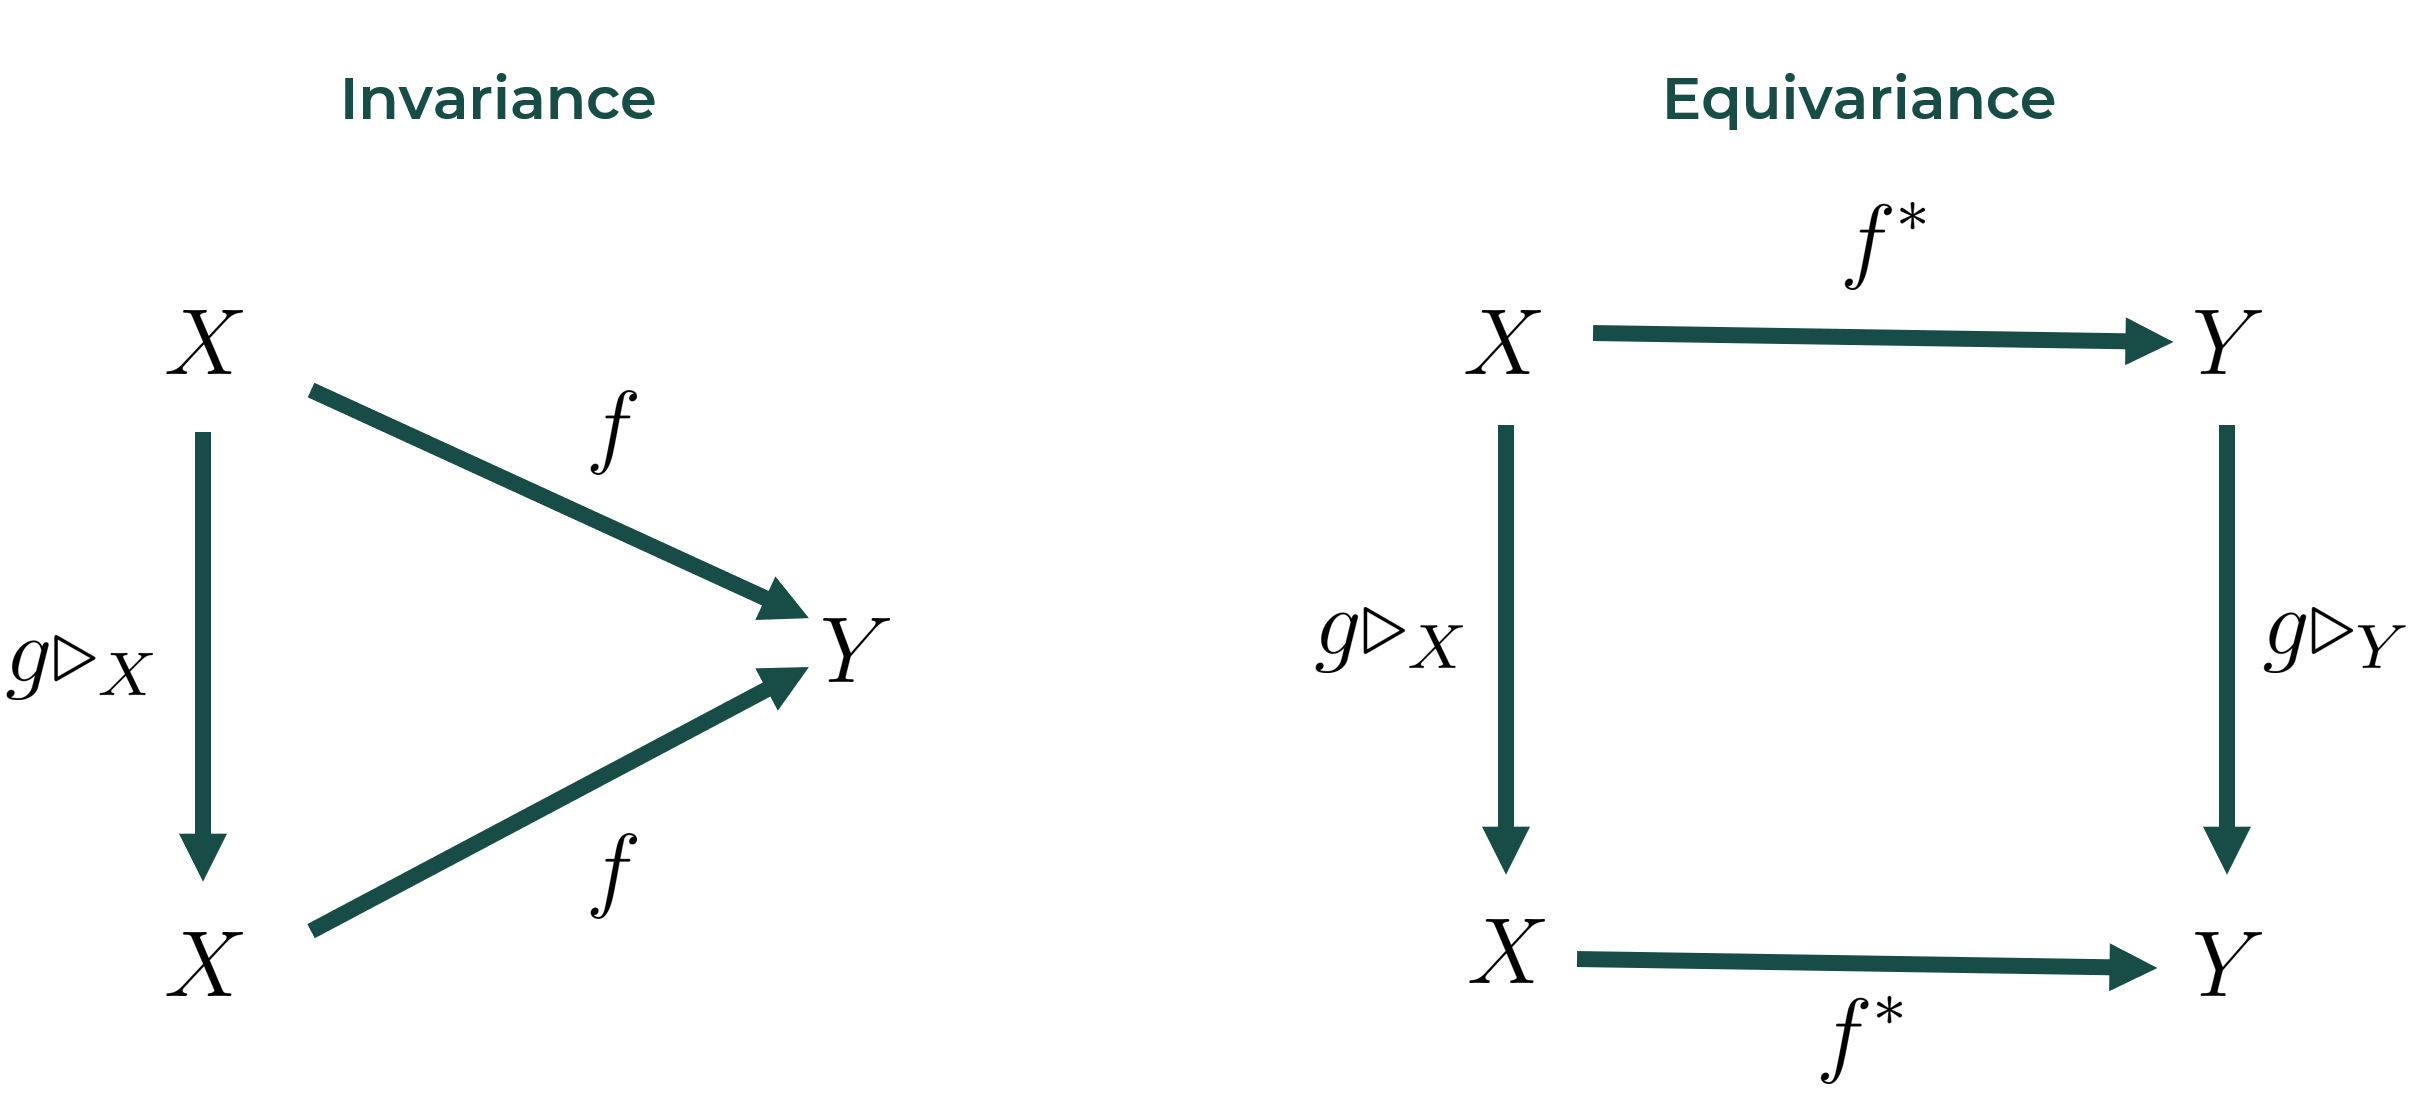
\includegraphics[width=0.9\textwidth]{Figure/Chapter 2/equivariance_1.png}
\caption{\label{fig:eqv1}
Diagrams show invariant and equivariant symmetry properties of functions $f$ and $f^{\ast}$ repectively.}
\end{figure}

The set of presumptions incorporated into a machine learning model that directs its learning process and enables it to more successfully generalise from sparse data is known as \textbf{inductive bias}.
Physical symmetries as inductive biases improve model accuracy and efficiency in the context of machine learning for atomic and molecular systems \cite{Langer2022,Meyer2023,Langer2024}.

Using \textbf{Equivariant descriptors}, which imposes symmetry requirements like rotational, translational, and permutational invariance directly inside the model architecture, is an effective strategy.
Equivariant models increase generalisation to unseen configurations and minimise the requirement for huge datasets by guaranteeing that the learnt representations follow these basic physical symmetries.
This requires the understanding of the equivariance idea which is the symmetry property but different from invariance.

Let consider a map 
\[f:X\rightarrow Y\]
which function $f$ maps any input $x\in X$ into $y\in Y$.
We need to consider a symmetry group $G$, e.g. permutation, reflection, or rotation group.
In the case of invariance we need a group action on space $X$.
Given a group element $g\in G$, the group action on any $x\in X$ can be written as $g\triangleright_{X}x$.
We can then state the function $f$ being \textbf{G-invariant} with respect to this action when the function satisfies 
\[f(g\triangleright_{X}x)=f(x)\quad\quad\forall g\in G,\;x\in X.\]
This means any transformed input is mapped to the same result and is depicted as the left diagram in Fig. \ref{fig:eqv1}.

In the case of equivariance, we need another a group action on space $Y$.
It can be written similarly as $g\triangleright_{Y}y$.
The function $f^{*}$ is then said to be \textbf{G-equivariant} with respect to the actions (on space $X$ and $Y$) when the function satisfies
\[f^{*}(g\triangleright_{X}x)=g\triangleright_{Y}f^{*}(x)\quad\quad\forall g\in G,\;x\in X.\]
This is illustated as the right diagram in Fig. \ref{fig:eqv1}.

\begin{figure}
\centering
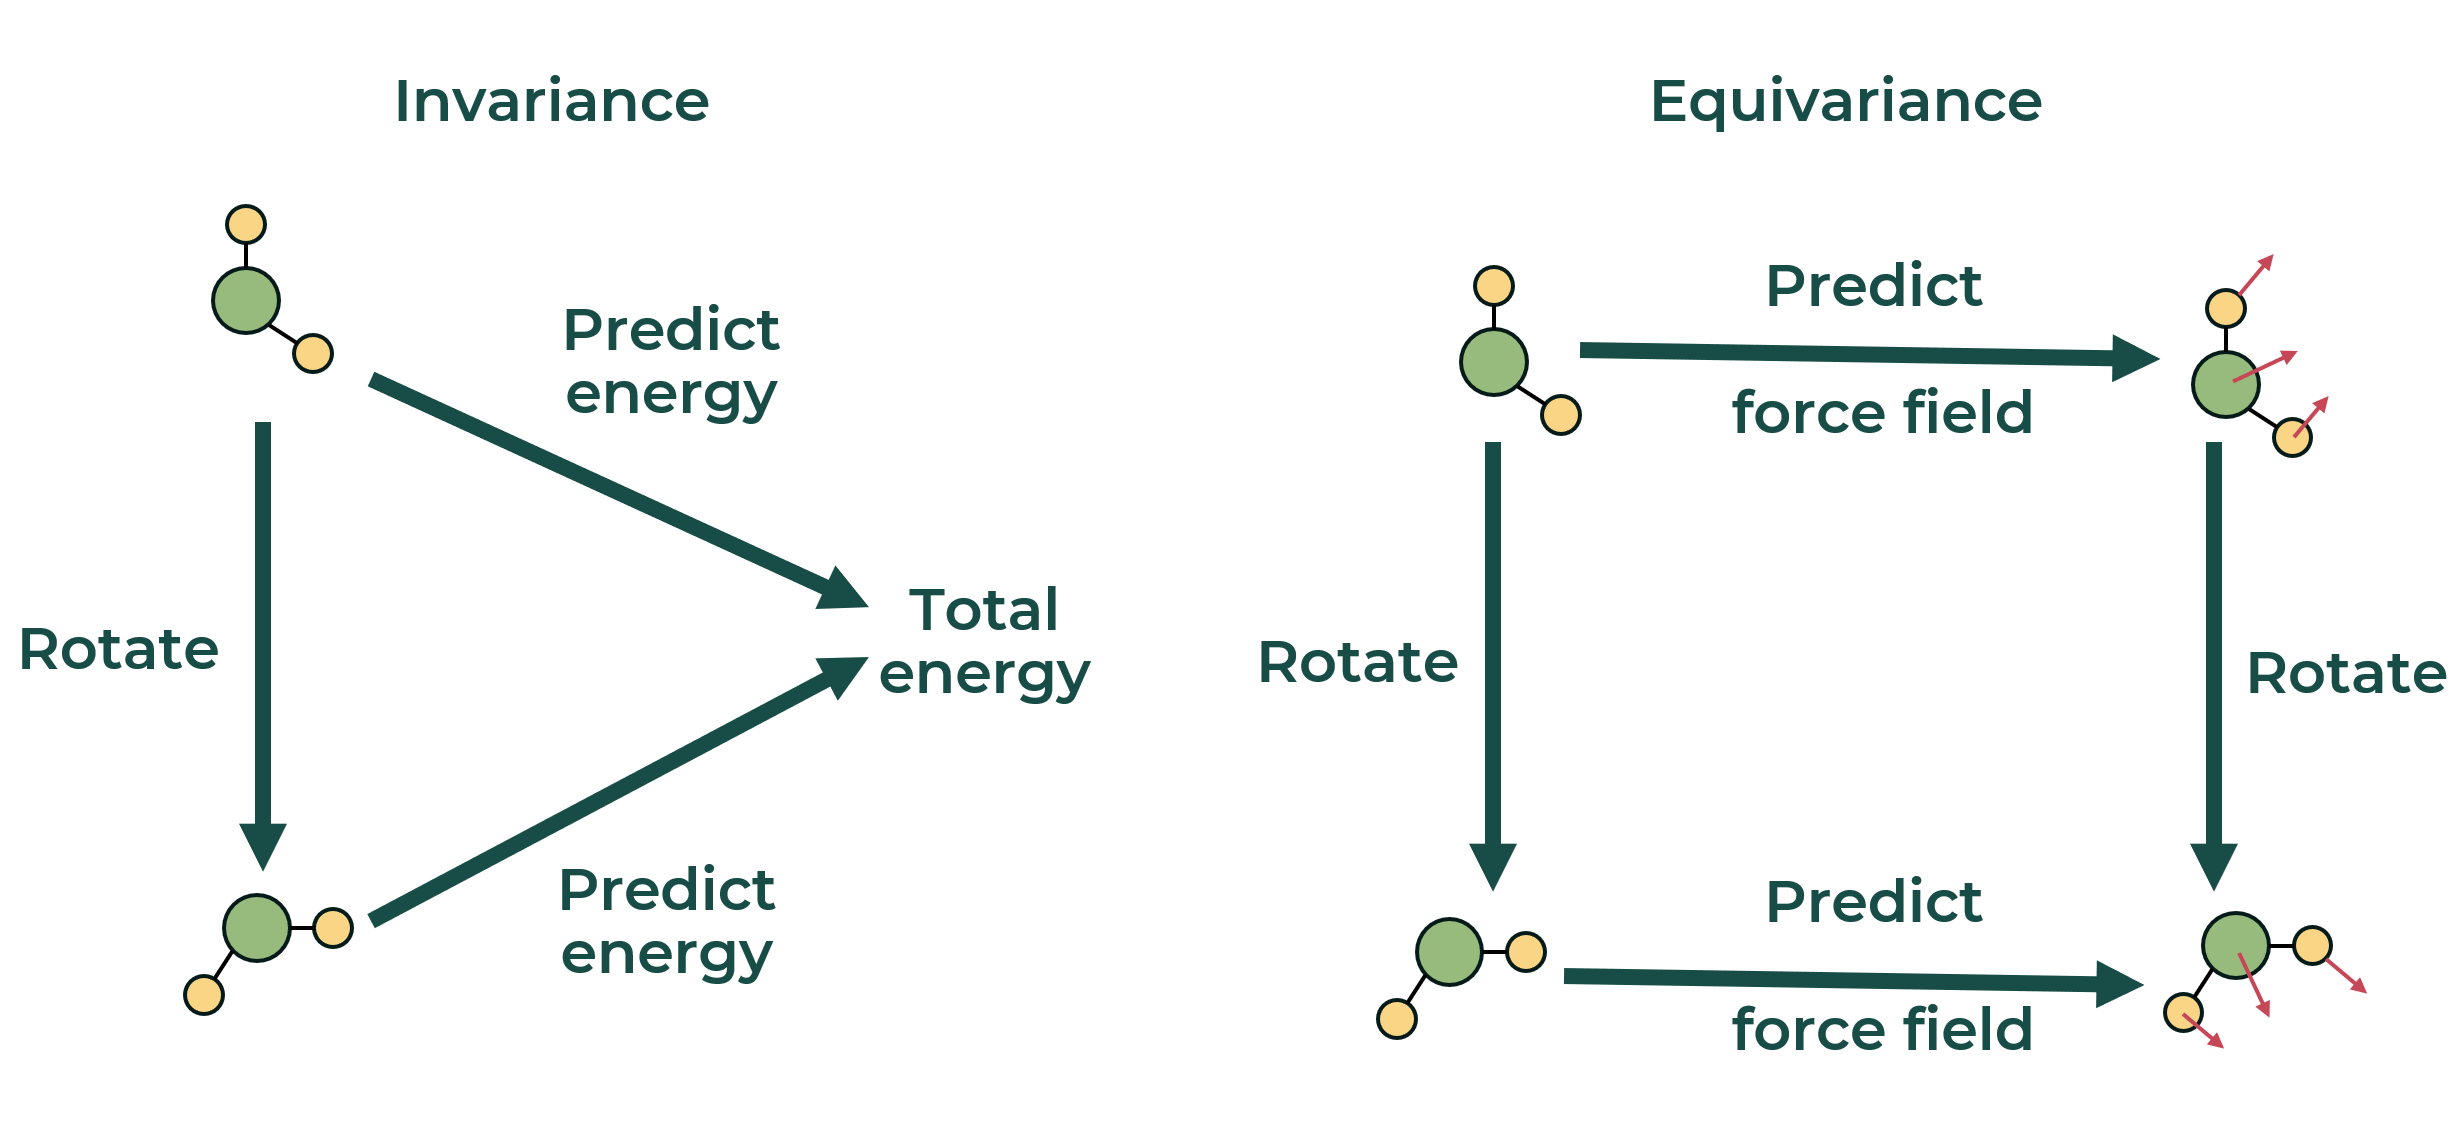
\includegraphics[width=0.9\textwidth]{Figure/Chapter 2/equivariance_2.png}
\caption{\label{fig:eqv2}
Examples of the invariance and equivariance for the prediction of a molecule’s properties.}
\end{figure}

In atomistic modelling, this distinction can be understood intuitively (Fig. \ref{fig:eqv2}).
Predicting a molecule’s total energy is an invariant task (left), since the scalar energy does not change under rotations or translations, whereas predicting a force field is an equivariant task, since the vector forces must rotate in step with the molecule (right).

We discuss how these ideas can be used to create machine learning potentials that faithfully represent interatomic interactions while preserving physical consistency in the following subsections.

\subsection{Reviews on Atomistic Descriptors} \label{subsec:2.4.1}
A recent assessment of several descriptors used in machine learning potential models was conducted by Langer et al. \cite{Langer2022}.
These descriptors fall into two general categories in the context of atomistic systems: local descriptors, which describe specific atomic surroundings \cite{Bartk2013}, and global descriptors, which depict the overall structure of the system.

For modelling local descriptors that rely solely on a finite-size atomic environment, such as forces, nuclear magnetic resonance (NMR) shifts, and core-level excitations \cite{Behler2007, Rupp2015}, local representations are especially well suited.
With additive approximations, which get system-wide attributes by adding up atomic contributions \cite{Himanen2020}, extensive global properties, like total energy, can also be modeled using local descriptors.
Since local descriptors only rely on a finite atomic environment rather than the whole system, they can be applied immediately to both finite and periodic systems without requiring any adaptation.
Examples of local atomistic descriptors are \textbf{Atom-Centred Symmetric Functions: ACSF} \cite{Behler2007,Behler2011}; \textbf{Smooth Overlap Atomic Positions: SOAP} \cite{Bartk2013,Bartk2015,Deringer2021}; \textbf{(Multi) Atomic Cluster Expansion: (M)ACE} \cite{Drautz2019, Musil2021, Dusson2022, Witt2023}; and the \textbf{Message Passing (MP)} version of \textbf{ACE}, \textbf{MACE} \cite{https://doi.org/10.48550/arxiv.2206.07697, Batatia2025}.

Note that \textbf{MACE} is, however, not a purely descriptor-based model in the traditional sense. While it builds on the ACE formalism for its functional basis, it embeds this within a neural message-passing architecture in which the effective descriptors and their weights are learned jointly from data rather than fixed a priori.

Global descriptors, which can represent either finite systems (molecules and clusters) or periodic systems (2D and 3D crystals), are designed to capture system-wide features such as the band gap, total energy, and polarisability tensor.
Examples for finite systems are \textbf{Coulomb Matrix: CM} \cite{Rupp2012}, and \textbf{Bag of Bonds: BoB} \cite{Hansen2015}, while \textbf{Many-body tensor representation: MBTR} \cite{Huo2022} can be employed for both finite and periodic systems.
Since periodic systems are consider as an infinite system, global descriptors need to be specially created or modified to take into consideration the boundary conditions and repeating nature of the system.

These descriptors meet the requirements of Quantum Mechanics / Machine Learning (QM/ML), except for \textbf{CM} \cite{Musil2021, Langer2022}.
The primary requirement is (1) \textit{Permutational, Translational, and Rotational Invariance}, as the descriptors of the atomistic system should remain unchanged under atom reordering, spatial translation, and rigid 3D rotation.

For interpolation, learning stability, and facilitating gradient-based learning and optimization, descriptors should be smooth functions of atomic positions and differentiable with respect to them. 
The second prerequisite—(2) \textit{Smoothness, Continuity, and Differentiability}—follows from this.
The comparison of these descriptors relied on those transformations and smoothness is illustrated in Table \ref{tab:2.1}.

The ability of QM/ML descriptors to discriminate between various atomistic structures in a unique way, hence avoiding degeneracies, is guaranteed by the third condition, (3) \textit{Uniqueness \& Completeness}.
In addition, they must have enough knowledge to precisely recreate material properties while preserving crucial physical aspects.
Completeness is necessary, but so is the fourth condition, (4) \textit{Compactness \& Efficiency}. Descriptors should encode all pertinent information required for precise predictions while remaining low-dimensional and computationally efficient.
The last prerequisite is (5) \textit{Scalability}, which means that descriptors must effectively scale with system size to be feasible for high-throughput simulations and large systems.%massive atomistic datasets.
Requirements (3)-(5) of those descriptors are compared in Table~\ref{tab:2.2}.

\textbf{ACE} and \textbf{MACE} descriptors rank among the top options for atomistic simulations, based on our comparison.
Yet, since message passing introduces non-linear scaling, \textbf{MACE} might be less efficient than \textbf{ACE}.
As these descriptors meet all necessary conditions—invariance, smoothness, uniqueness, efficiency, and scalability—and provide linear scaling with system size, they are extremely useful for large-scale atomistic simulations.
Since \textbf{SOAP} descriptors are the foundation for the development of \textbf{ACE} models, it is crucial to introduce them in the context of \textbf{Gaussian Approximation Potentials (GAP)} before diving into the mathematical underpinnings of \textbf{ACE} models.
The following subsection will examine this.

\subsection{GAP \& SOAP} \label{subsec:2.4.2}
%Machine learning plays an essential role when it applies to solving quantum mechanical challenges.  It makes it easier to solve Sch\"{o}dinger's and Dirac's equations, which makes it possible to calculate potential energy surfaces for both atomistic and coarse-grained systems with accuracy. 
Understanding material properties and chemical interactions requires accurate energy calculations in these systems, which include bulk crystals, surfaces, atomic clusters, and molecules.
Potential energy datasets derived from DFT calculations are examples of reference electronic structure computations that may be used to predict potential energy surfaces by utilising machine learning. These predictions can be made without the need for detailed physical interpretations \cite{Bartk2010} if the dataset is large enough.

Many effective machine learning potential approaches have been developed in the last ten years. 
A. P. Bartók et al. (2010) introduced the \textbf{Gaussian Approximation Potential (GAP)} \cite{Bartk2010, Bartk2015}, which is a particularly noteworthy approach as the foundation of the current succesful approches, such as a \textbf{(M)ACE} model \cite{Drautz2019, Dusson2022, Witt2023, Batatia2025}.

%\newpage
\begin{landscape}
\begin{longtable}[c]{|l|lll|l|}
\hline
\multicolumn{1}{|c||}{\multirow{2}{*}{\textbf{Desc.}}} &
  \multicolumn{3}{c|}{{\textbf{Invariance}}} &
  \multicolumn{1}{c|}{\textbf{Smoothness, Continuity,}} 
  \\ \cline{2-4}
\multicolumn{1}{|c||}{} &
  \multicolumn{1}{c|}{\textbf{Permutation}} &
  \multicolumn{1}{c|}{\textbf{Translation}} &
  \multicolumn{1}{c|}{\textbf{Rotation}} &
  \multicolumn{1}{c|}{\textbf{\& Differentiability}} 
  \\ \hline
\endfirsthead
%
\endhead
%
\multicolumn{1}{|c||}{ \textbf{CM} } &
  \multicolumn{1}{l|}{
    \begin{tabular}[c]{@{}l@{}} 
        \textbf{Yes} \\
        (Require sorting)
    \end{tabular}
        }&
    \multicolumn{1}{l|}{
    \begin{tabular}[c]{@{}l@{}}
        \textbf{No}
    \end{tabular}
    }&
    \multicolumn{1}{l|}{
    \begin{tabular}[c]{@{}l@{}}
        \textbf{No}
    \end{tabular}
    }&
    \multicolumn{1}{l|}{\textbf{No}}
    \\ \hline
    
\multicolumn{1}{|c||}{\textbf{BoB} } &
    \multicolumn{1}{l|}{
    \begin{tabular}[c]{@{}l@{}} 
        \textbf{Not Fully} \\
        (Require sorting)
    \end{tabular}
    }&
    \multicolumn{1}{l|}{
    \begin{tabular}[c]{@{}l@{}}
        \textbf{Not Fully} (Require \\
        explicit translational \\
        symmetry )
    \end{tabular}
    }&
    \multicolumn{1}{l|}{
    \begin{tabular}[c]{@{}l@{}}
        \textbf{No}
    \end{tabular}
    }&
    \multicolumn{1}{l|}{\textbf{No}}
    \\ \hline
    
\multicolumn{1}{|c||}{\textbf{MBTR} } &
  \multicolumn{1}{l|}{
    \begin{tabular}[c]{@{}l@{}} 
        \textbf{Not Inherently}\\
        (Approximated via \\
        kernel methods)
    \end{tabular}
    }&
    \multicolumn{1}{l|}{
    \begin{tabular}[c]{@{}l@{}}
        \textbf{Not Inherently} \\
        (Approximated\\
        using relative \\
        distances and angles)
    \end{tabular}
    }&
    \multicolumn{1}{l|}{
    \begin{tabular}[c]{@{}l@{}}
        \textbf{Not Fully} (Depending \\
        on chosen coordinate \\
        system.)
    \end{tabular}
    }&
    \multicolumn{1}{l|}{
    \begin{tabular}[c]{@{}l@{}}
        \textbf{Yes} (Using smooth \\
        kernel functions.)
    \end{tabular}
    }
    \\ \hline

\multicolumn{1}{|c||}{\textbf{ACSF} } &
  \multicolumn{1}{l|}{
    \begin{tabular}[c]{@{}l@{}} 
        \textbf{Yes} (Summing\\
        over local ACSFs)
    \end{tabular}
    }&
    \multicolumn{1}{l|}{
    \begin{tabular}[c]{@{}l@{}}
        \textbf{Locally Yes} \\
        (Only considering \\
        locally relative \\
        atomic distances)
    \end{tabular}
    }&
    \multicolumn{1}{l|}{
    \begin{tabular}[c]{@{}l@{}}
        \textbf{Not Fully} (Radial SFs \\
        are invariant, but \\
        angular SFs are not fully\\
        rotation-independent.)
    \end{tabular}
    }&
    \multicolumn{1}{l|}{
    \begin{tabular}[c]{@{}l@{}}
        \textbf{Yes} (Employing\\
        analytical radial\\ 
        and angular functions.)
    \end{tabular}
    }
    \\ \hline

\multicolumn{1}{|c||}{\textbf{SOAP} } &
  \multicolumn{1}{l|}{
    \begin{tabular}[c]{@{}l@{}} 
        \textbf{Fully}
  \end{tabular}
  }&
  \multicolumn{1}{l|}{
    \begin{tabular}[c]{@{}l@{}}
  \textbf{Yes} (Based on \\
  local atomic density) 
  \end{tabular}
  }&
  \multicolumn{1}{l|}{
    \begin{tabular}[c]{@{}l@{}}
  \textbf{Yes} (Using\\
  spherical harmonics)  
  \end{tabular}
  }&
  \multicolumn{1}{l|}{\textbf{Fully}}\\ \hline

\multicolumn{1}{|c||}{\textbf{ACE} } &
  \multicolumn{4}{c|}{
  \textbf{Fully}
  }
  \\ \hline
  
\multicolumn{1}{|c||}{\textbf{MACE} } &
  \multicolumn{4}{c|}{
  \textbf{Fully}
  }
  \\ \hline
\caption{\label{tab:2.1} Comparison of atomic descriptors based on invariance properties and smoothness.} \\
\end{longtable}
\end{landscape}
% Left and right margin adjustments
\begin{landscape}
\begin{longtable}[c]{|l|l|l|l|l|l|}
\hline
\multicolumn{1}{|c||}{\multirow{2}{*}{\textbf{Desc.}}} &
\multicolumn{1}{c|}{\multirow{2}{*}{\textbf{Uniqueness}}} &
\multicolumn{1}{c|}{\multirow{2}{*}{\textbf{Completeness}}} &
\multicolumn{1}{c|}{\textbf{Compactness}} &
\multicolumn{1}{c|}{\multirow{2}{*}{\textbf{Scalability}}} \\
\multicolumn{1}{|c||}{} &
\multicolumn{1}{c|}{\textbf{}} &
\multicolumn{1}{c|}{\textbf{}} &
\multicolumn{1}{c|}{\textbf{\& Efficiency}} &
\multicolumn{1}{c|}{\textbf{}}\\ \hline
\endfirsthead
%
\endhead
%
\multicolumn{1}{|c||}{ \textbf{CM} } &
  \multicolumn{1}{l|}{
    \begin{tabular}[c]{@{}l@{}} 
        \textbf{No}
    \end{tabular}
        }&
    \multicolumn{1}{l|}{
    \begin{tabular}[c]{@{}l@{}}
       \textbf{ No}
    \end{tabular}
    }&
    \multicolumn{1}{l|}{
    \begin{tabular}[c]{@{}l@{}}
        \textbf{Compact} \& \textbf{Efficient}
    \end{tabular}
    }
    &
    \multicolumn{1}{c|}{
    $\mathcal{O}(N^2)$
    }
    \\ \hline
  
\multicolumn{1}{|c||}{\textbf{BoB} } &
  \multicolumn{1}{l|}{
    \begin{tabular}[c]{@{}l@{}} 
        \textbf{No}
    \end{tabular}
        }&
    \multicolumn{1}{l|}{
    \begin{tabular}[c]{@{}l@{}}
        \textbf{No}
    \end{tabular}
    }&
    \multicolumn{1}{l|}{
    \begin{tabular}[c]{@{}l@{}}
        \textbf{More Compact} \& \textbf{Efficient} \\
        than \textbf{CM}
    \end{tabular}
    }
    &
    \multicolumn{1}{c|}{
    $\mathcal{O}(N^2)$
    }
    \\ \hline
  
\multicolumn{1}{|c||}{\textbf{MBTR}} &
  \multicolumn{1}{l|}{
    \begin{tabular}[c]{@{}l@{}} 
        \textbf{Yes} (Using multi-body\\
        correlations)
    \end{tabular}
        }&
    \multicolumn{1}{l|}{
    \begin{tabular}[c]{@{}l@{}}
        \textbf{Yes} (Rely on the kernel\\
        choices)
    \end{tabular}
    }&
    \multicolumn{1}{l|}{
    \begin{tabular}[c]{@{}l@{}}
        \textbf{Less Compact \& Expensive}\\
        (Descriptors grow quickly\\
        with complexity) \\
    \end{tabular}
    }
    &
    \multicolumn{1}{c|}{
    $\mathcal{O}(N^3)$
    }
    \\ \hline
  
\multicolumn{1}{|c||}{\textbf{ACSF} } &
  \multicolumn{1}{l|}{
    \begin{tabular}[c]{@{}l@{}} 
        \textbf{Not guaranteed to be Unique.} \\
        (Different local environments \\
        can have similar \textbf{SFs}, leading \\
        to possible degeneracies.
    \end{tabular}
        }&
    \multicolumn{1}{l|}{
    \begin{tabular}[c]{@{}l@{}}
        \textbf{Not guaranteed to be} \\
        \textbf{Complete} (Certain \\
        atomic environments \\
        can map to same \textbf{ACSF}.
    \end{tabular}
    }&
    \multicolumn{1}{l|}{
    \begin{tabular}[c]{@{}l@{}}
        \textbf{Compact \& Efficient} (Local \\
        descriptors controlled by \textbf{SF} \\
        parameters \& independently \\
        evaluated)
    \end{tabular}
    }&
    \multicolumn{1}{c|}{
    $\mathcal{O}(N)$
    }
    \\ \hline
  
\multicolumn{1}{|c||}{\textbf{SOAP} } &
  \multicolumn{1}{l|}{
    \begin{tabular}[c]{@{}l@{}} 
        \textbf{Fully}
    \end{tabular}
        }&
    \multicolumn{1}{l|}{
    \begin{tabular}[c]{@{}l@{}}
        \textbf{Complete}\\
        (Tractable in lower \\
        body-order expansions)
    \end{tabular}
    }&
    \multicolumn{1}{l|}{
    \begin{tabular}[c]{@{}l@{}}
        \textbf{Less Compact \& Moderately}\\
        \textbf{Efficient} (Depend on radial/\\
        angular resolution)
    \end{tabular}
    }&
    \multicolumn{1}{c|}{
    $\mathcal{O}(N^2)$
    }
    \\ \hline
  
\multicolumn{1}{|c||}{\textbf{ACE} } &
  \multicolumn{1}{l|}{
    \begin{tabular}[c]{@{}l@{}} 
        \textbf{Fully} 
    \end{tabular}
        }&
    \multicolumn{1}{l|}{
    \begin{tabular}[c]{@{}l@{}}
        \textbf{Fully} (only to the chosen \\
        body-order)
    \end{tabular}
    }&
    \multicolumn{1}{l|}{
    \begin{tabular}[c]{@{}l@{}}
        \textbf{Compact \& Highly Efficient}
    \end{tabular}
    }&
    \multicolumn{1}{c|}{
    $\mathcal{O}(N)$
    }
    \\ \hline
  
\multicolumn{1}{|c||}{\textbf{MACE} } &
  \multicolumn{1}{l|}{
    \begin{tabular}[c]{@{}l@{}} 
        \textbf{Fully} 
    \end{tabular}
        }&
    \multicolumn{1}{l|}{
    \begin{tabular}[c]{@{}l@{}}
        \textbf{Fully} (only to the chosen \\
        body-order)
    \end{tabular}
    }&
    \multicolumn{1}{l|}{
    \begin{tabular}[c]{@{}l@{}}
        \textbf{Compact} but \textbf{Less Efficient}\\
        than \textbf{ACE} (Using MP)
    \end{tabular}
    }&
    \multicolumn{1}{c|}{
    $\mathcal{O}(N)$
    }
    \\ \hline
\caption{\label{tab:2.2} Comparison of atomic descriptors based on uniqueness, completeness, compactness, and scalability.} \\ 
\end{longtable}
\end{landscape}

\newpage

By representing an $N$-atomic system's overall energy as the sum of its local atomic contributions, this method simulates the interatomic potential of that system.
The total energy is expressed by
\begin{equation}
    \label{equ:2.46}
     E_{\text{tot}} = \sum_{\alpha\in p,t}\sum_{j\:\in\:\alpha}\epsilon_{j}^{\alpha} + \mathcal{V}_{\text{long range}}.
\end{equation}
This atomic system's total energy is represented by the sum of its short- and long-range terms \cite{Bartk2015, Bartk2013, Deringer2021}. 
Electrostatic Van der Waals and polarisability contributions are included in the long-range term.
The local energy functional contributions inside a certain cutoff radius, which makes up the short-range term.
The local contributions within this cutoff zone are classified into various categories, $\alpha$, based on suitable atomic descriptors.
Pair distances for two-body interactions ($p$) and bond angles for three-body interactions ($t$)%, and dihedral angles for four-body interactions 
are examples of these descriptors.
The index $j$, which is the sum over the bonds, the bond angles, or the dihedral angles in the system, is used to index each contribution.

Because the GAP framework is additive and local, the approach typically neglects long-range contributions and only includes low-order cluster expansion terms. 
Consequently, the total energy function's general form can be reduced to
\begin{equation}
    \label{equ:2.47}
     E^{\text{GAP}}_{\text{tot}} = \sum_{p\:\in\:\forall\:\text{pairs}}\epsilon_{p}^{(2)} + \sum_{t\:\in\:\forall\:\text{triplets}}\epsilon_{t}^{(3)},
\end{equation}
where $\epsilon_{p}^{(2)}$ and $\epsilon_{t}^{(3)}$ correspond to two- and three-body contributions.

We can reformulate the system's total energy using an atom-centered method. This method specifies the local atomic environment of each $i^{\text{th}}$ atom by positioning it at the centre of a cutoff zone. The nearby atoms in this area are then used to build the atomic descriptors.

The Cartesian coordinates of nearby atoms are transformed into a modified descriptor using a transformation function to represent the local energy contribution of each $i^{\text{th}}$ atom. This change guarantees that the local energy can only be determined by the relative positions of the atoms in the cutoff radius.  

The system's total energy can be rewritten as follows using this atom-centered framework:
\begin{equation}
    \label{equ:2.48}
     E^{\text{GAP}}_{\text{tot}} = \sum^{\text{atoms}}_{i}\epsilon^{i}(\textbf{d}_{i}),
\end{equation}
where $\textbf{d}_{i}$ is the $i^{\text{th}}$ atomic descriptor.
In the \textbf{GAP} framework, the local energy $\epsilon^{i}$ is expressed as a sum of arbitrary basis functions $\phi_{m}$ of the descriptor $\textbf{d}_{i}$.
This descriptor, more explicitly, represents the coordinates of the atom $i$ surrounded by its neighbour atoms. 
This local energy can be written as
\begin{equation}
    \label{equ:2.49}
     \epsilon^{i}(\textbf{d}_{i})= \textbf{c}^{\text{T}}\Phi = \sum_{m\:=\:1}^{d}c_{m}\phi_{m}(\textbf{d}_{i}),
\end{equation}
where $c_{m}$ is the weight parameters of a $d$-dimensional weight vector $\textbf{c}$ corresponding to basis functions $\phi_{m}$ of the basis vector $\Phi$. 
If each of the weights follows a zero-mean Gaussian distribution, i.e. 
\[\textbf{c}\sim\mathcal{N}_{d}(\textbf{c};\:\textbf{0},\:\sigma_{c}\mathbb{I}),\]
then the equation above naturally extends to a Gaussian process (GP).
The primary objective of \textbf{GAP} is to employ a GP model for predicting atomic energies based on arbitrary descriptors. 
This prediction is performed using a pre-training dataset obtained from electronic structure calculations, enabling accurate and data-efficient modelling of interatomic interactions.

Employing a GP requires defining similarity measures between two atomic descriptors through a kernel function, $k(\textbf{d}_{i},\:\textbf{d}_{j})$.
This kernel function measures the correlation between two atomic environments, in order to guarantee that structurally similar configurations produce similar predicted energies.
The kernel function can be constructed using the covariance between two atomic energies, \( \langle \epsilon^{i} \epsilon^{j} \rangle \). This relationship, as deduced in \cite{Bartk2015}, results in:
\begin{equation}
    \label{equ:2.50}
    k(\textbf{d}_{i},\:\textbf{d}_{j}) = \sum_{m\:=\:1}^{d}\phi_{m}(\textbf{d}_{i})\phi_{m}(\textbf{d}_{j}).
\end{equation}
This kernel function must be reconstructed to a covariance matrix for predicting the \textit{local} atomic energy $\epsilon^{\star}$ of a descriptor $\textbf{d}^{\star}$ from a pre-training dataset $\textbf{E}$. 
If a pre-training dataset $\textbf{E}= \left[\epsilon^{1}\:\epsilon^{2}\cdots\epsilon^{n} \right]^{\text{T}}$ contains $n$ \textit{local} atomic energies corresponding to individual $n$ atomic descriptors in the set of descriptors $\textbf{D}= \left[\textbf{d}_{1}\:\textbf{d}_{2}\cdots\textbf{d}_{n} \right]^{\text{T}}$, the $n\times n$ covariance matrix over the pre-training dataset is defined as $K(\textbf{D}) \propto \langle \textbf{E}\textbf{E}^{\text{T}} \rangle$. 
The predicting posterior mean of the atomic energy, analogous to Eq. (\ref{equ:2.36}), can be calculated from 
\begin{equation}
    \label{equ:2.51}
    \overline{\epsilon}^{\star} = k(\textbf{d}^{\star},\:\textbf{D})\cdot K^{-1}(\textbf{D})\cdot\textbf{E},
\end{equation}
where $k\propto\langle \epsilon^{\star}\textbf{E}\rangle$ is the covariance of between the posterior atomic energy and prior atomic energies.

Using a GP model to predict the \textit{local} atomic energy proves to be a highly effective approach.
The prediction relies solely on a set of prior atomic energies obtained from electronic structure calculations and a kernel function that measures the similarity between different descriptors.
Unlike traditional methods such as empirical interatomic potentials or cluster expansion methods, there is no need to explicitly define basis functions or determine the corresponding weights.
Furthermore, this implies that physical interpretation and understanding are not strictly required to achieve accurate energy predictions.

Although a GP model does not require explicit physical understanding, achieving accurate predictions can be computationally expensive.
Since the model is not inherently constrained by underlying physical symmetries and conservation laws, it must learn these properties directly from data through a data-driven approach.
This requires training on a large dataset of total energies and forces to capture the correct physical behavior.
Consequently, the number of training datapoints can reach tens of thousands to achieve acceptable predictive accuracy.

To minimize the number of required electronic structure calculations, physical symmetries of the system can be incorporated into the GP model before training.
Specifically, the choice of atomic descriptors can be designed to inherently satisfy these symmetries or, mathematically, to serve as representations of the corresponding symmetry groups.
By embedding these symmetry-aware descriptors as an inductive bias, the model's predictive accuracy is enhanced while reducing the dependence on large training datasets.

Bart\'{o}k and Cs\'{a}nyi et al., using the Smooth Overlap of Atomic Positions (SOAP) framework, presented a methodical way to choose a suitable description for a GAP model \cite{Bartk2013, Bartk2015}.
In Cartesian coordinates, they first define the atomic descriptor for atom $i$ as a density function that represents its immediate atomic environment, expressed as 
\begin{equation}
    \label{equ:2.52}
      \rho_{i}(\mathbf{r}) = \sum_{j}^{\text{neigh.}} 
      \exp\!\left(-\frac{\lVert\mathbf{r}-\mathbf{r}_{ij}\rVert^{2}}{2\sigma^{2}}\right),
\end{equation}
This neighbour density includes Gaussian peaks specifying the spatial distribution of neighboring atoms $j$.
The centre of the neighboring peaks is displaced from atom $i$ by the relative position $\textbf{r}_{ij}$, capturing the atomic environment in a smooth and differentiable manner.
We can employ this neighbour density to rewrite Equation (\ref{equ:2.49}) in terms of atomic energy $\epsilon^{i}$ as a functional of the atomic density $\rho_{i}$,
\begin{equation}
    \label{equ:2.53}
      \epsilon^{i}[\rho_{i}] = \int c(\textbf{r})\rho_{i}(\textbf{r})d\textbf{r},
\end{equation}
where the weight $c$ is also Gaussian distributed.
Evaluating the covariance $\langle\epsilon^{i}\epsilon^{j}\rangle$ then defines the kernel function as 
\begin{equation}
    \label{equ:2.54}
      k(\rho_{i}, \rho_{j}) = \int \rho_{i}(\textbf{r})\rho_{j}(\textbf{r})d\textbf{r}.
\end{equation}
By integrating all the associated density functions, this formulation guarantees that the kernel function captures the similarity between atomic environments. However, this kernel function is not invariant under 3D rotations due to the chosen neighbour density $\rho_{i}$. 

To ensure rotational invariance, the density function in Equation (\ref{equ:2.52}) can be re-expanded in terms of radial and spherical basis functions to form a \textbf{single particle basis function} as follows,
\begin{equation}
    \label{equ:2.55}
      \rho^{(i)}(\textbf{r}) = \sum_{nlm}
      c^{(i)}_{nlm}
      R_{nl}(r)Y^{m}_{l}(\hat{\textbf{r}}),\quad\quad n,\;l\in\mathbb{N},\;m\{-l,\cdots,l\},
\end{equation}
where $\textbf{r}=r\hat{\textbf{r}}$ and $c^{(i)}_{nlm}$ are the coefficients of the expansion for atom $i$.
$R_{nl}(r)$ is a radial basis function depending on the magnitude of vector $\textbf{r}$ and $Y^{m}_{l}$ is a spherical harmonic basis function depending on the direction of vector $\textbf{r}$.

To use the spherical density function, not only can it be substituted in the above kernel function, it can be used in the form of a \textbf{power spectrum} defined as
\begin{equation}
    \label{equ:2.56}
P^{(ij_{1})}_{n l} = \sum^{l}_{m = -l} c^{(i)}_{nlm} \left(c^{(j_{1})}_{nlm}\right)^{*},
\end{equation}a
which captures two-body correlations and serving as the standard SOAP descriptor in \textbf{GAP}.
The crucial property of Equation~\eqref{equ:2.56} is that the sum over the magnetic quantum numbers \(m\) corresponds to integrating over all possible rotations (i.e. averaging over the orthogonal group \(\mathrm{O}(3)\) with respect to the Haar measure).
As a result, the power spectrum coefficients are invariant under any 3D rotation of the atomic environment, even though the underlying neighbour density \(\rho_{i}(\mathbf{r})\) is not.

To capture three-body correlations, the \textbf{Bispectrum}, defined as
\begin{equation}
    \label{equ:2.57}
B^{(ij_{1}j_{2})}_{n_1 l_1 n_2 l_2 l} = \sum_{m_1 m_2} C_{l_1 m_1 l_2 m_2}^{l m} c^{(i)}_{n_1 l_1 m_1} \left(c^{(j_{1})}_{n_1 l_1 m_1}\right)^{*}  c^{(j_{2})}_{n_2 l_2 m_2},
\end{equation}
incorporates Clebsch-Gordan coefficients \( C_{l_1 m_1 l_2 m_2}^{l m} \) between two spherical harmonic components.
This coupling requires the tensor product of two density functions in Equation ~\eqref{equ:2.55} leading to more expensive computation than \textbf{power spectrum}.
While the \textbf{power spectrum} efficiently captures structural features and is widely used in GAP, the \textbf{bispectrum} provides richer information at the cost of increased complexity.
The computational complexity increases factorially with the body order due to the coupling of multiple density components.
However, these decompositions make the descriptor more appropriate for machine learning models that adhere to basic physical symmetries by guaranteeing that it stays invariant under 3D rotations.
The derivations of these decompositions are stated in \cite{,Bartk2013,Deringer2021}.

Regarding the power spectrum and bispectrum, we can express the energy of atom $i$ with its environment as follows
\begin{equation}
    \label{equ:2.58}
      \epsilon^{i} = \sum_{j_{1}}\sum_{k_{1}}
      \tilde{c}_{k_{1}}
      P^{(ij_{1})}_{k_{1}} + \sum_{j_{1}\neq j_{2}}\sum_{k_{2}}
      \tilde{c}_{k_{2}}
      B^{(ij_{1}j_{2})}_{k_{2}}
      ,
\end{equation}
where $\tilde{c}_{k_{1}}$ and $\tilde{c}_{k_{2}}$ are the fitting coefficients indexed by quantum numbers $k_{1} = (n,\;l)$ and $k_{2} = (n_1,\;l_1,\;n_2,\;l_2,\;l)$ respectively. To obtain the total energy, we substitute the atomic energy back into Equations (\ref{equ:2.48}) and the result is equivalent to Equation (\ref{equ:2.47}).

To estimate the coefficients $\tilde{\mathbf{c}}=\{\tilde{c}_{k_{1}},\;\tilde{c}_{k_{2}}\}$ we consider a regularised least-squares loss function with a joint objective over observed total energies $\mathcal{E}^{\text{obs}}_{\textbf{x}}$, forces $\mathcal{F}^{\text{obs}}_{\textbf{x}}$, and virials (or stresses) $\mathcal{V}^{\text{obs}}_{\textbf{x}}$ for each structure $\textbf{x}$ in the training set $\mathcal{R}$. 
The objective can be expressed as
\begin{equation}
\label{equ:loss}
\begin{split}
\mathcal{L}(\tilde{\mathbf{c}})=
\sum_{\textbf{x}\in\mathcal{R}}\big(
&w_{E,\textbf{x}}^{2}\big\|E(\tilde{\mathbf{c}},\;\textbf{x})-\mathcal{E}^{\text{obs}}_{\textbf{x}}\big\|_2^2
+w_{F,\textbf{x}}^{2}\big\|F(\tilde{\mathbf{c}},\;\textbf{x})-\mathcal{F}^{\text{obs}}_{\textbf{x}}\big\|_2^2
\\&
+w_{V,\textbf{x}}^{2}\big\|V(\tilde{\mathbf{c}},\;\textbf{x})-\mathcal{V}^{\text{obs}}_{\textbf{x}}\big\|_2^2\big)
+R,
\end{split}
\end{equation}
where the weights $w_{E,\textbf{x}},\;w_{F,\textbf{x}},\;w_{V,\textbf{x}}$ allow differential emphasis on various observables, typically scaled with the number of atoms in each structure $R$ to balance the relative contributions of energies, forces, and virials.
The final term represents regularisation for prevent overfitting, occuring when a model learns noise or irrelevant details from the training data instead of capturing the underlying physical relationships. By adding a penalty term to the loss function, regularisation constrains the model parameters. The detail calculations are provided in section 2 of the Gaussian process review~\cite{Deringer2021}.

%Minimising the objective in Eq.~\eqref{equ:loss} yields the normal equations
%\begin{equation}
%\label{equ:loss_sol}
%\big(K_{MM}+K_{MN}\Sigma^{-1}K_{NM}\big)\tilde{\mathbf{c}}=K_{MN}\Sigma^{-1}\mathbf{y},
%\end{equation}
%where $\mathbf{y}$ collects all energy, force, and virial observations, $\Sigma$ encodes their respective weights, %and $K_{NM}$ denotes the cross-kernel matrix between training environments and representative environments.
%The analytic solution follows as
%\begin{equation}
%\label{equ:loss_coef}
%\tilde{\mathbf{c}}=\big(K_{MM}+K_{MN}\Sigma^{-1}K_{NM}\big)^{-1}K_{MN}\Sigma^{-1}\mathbf{y}.
%\end{equation}
%This formulation corresponds to a Gaussian process regression (GPR) model in which the regularisation term plays the role of a Gaussian prior on $\tilde{\mathbf{c}}$, and the joint inclusion of energy, force, and virial residuals ensures that the learned potential energy surface and its derivatives are fitted self-consistently.

In the next section, we will provide the extended framework to \textbf{GAP} for capturing up to a higher-order body term while maintaining a linear scaling with respect to body order. 
This computationally tractable framework is known as \textbf{Atomic Cluster Expansion (ACE)}.

%Additionally in SOAP, there is also the generalisation of the \textbf{power spectrum} concept to enlarge the set of the invariant functions through a \textbf{bispectrum} approach stated in \cite{,Bartk2013,Deringer2021}.

%These kernel methods are efficient for the prediction of scalar quantities such as potential energy surfaces of atomistic environments. However, there was the gap of generalised GPR models to predict non-scalar properties. These can be vectorial or tensorial properties caused by materials responding to mechanical, magnetic, or electrical perturbations. For instance, the electrical response moments can be dipole moments, polarizability, or hyperpolarizability. To predict these properties, kernels in the GPR method need to be body-ordered equivariant. 

%Regarding the recent work from Ceriotte's group \cite{Wigner-kernel}, they introduce one of the equivariant and body-ordered kernels, called \textbf{Wigner kernels}. These \textbf{Wigner kernels} scale superiorly with the size of an atomic environment since they avoid the expansion of their basis set to the radial and chemical type representation for the atomic environment. As written in equation \ref{eqution:2.6}, the standard GPR model 
%\newpage
\section{Atomic Cluster Expansion} \label{sec:2.5} \paragraph{}
In the previous section, we reviewed atomic descriptors used in machine learning potential models. We also discussed local atomistic descriptors, particularly \textbf{SOAP}, and its corresponding Gaussian process model (\textbf{GAP}).
This model employs a cluster expansion approach, expanding interactions up to the three-body order.
It is restricted to low-body orders because the descriptor's complexity scales factorially with increasing body order.
To overcome this limitation, the \textbf{Atomic Cluster Expansion (ACE)} framework is developed by Ralf Drautz in 2019 \cite{Drautz2019}, providing a more efficient descriptor which achieves linear scaling with the body order.

\subsection{Canonical Cluster Expansion} \label{sec:2.5.1}
In this section, we present a brief mathematical discussion constructing hte \textbf{ACE} model.
The first step is to reformulate the total energy in Equation~(\ref{equ:2.48}) as the sum of the site (atomic) energies \cite{Dusson2022, Witt2023,Drautz2019} as follows 
\begin{equation}
\label{equ:2.59}
E(\left\{ \mathbf{r}_{i}\right\}_{i=1}^{J}) 
= \sum_{i=1}^{J} \epsilon(\left\{ \mathbf{r}_{ij}\right\}_{j=1}^{J-1}),
\end{equation}
where $\mathbf{r}_{i}$ is the position of the centre atom $i$ and its atomic displacement, from its neighbouring atom $j$, is defined as $\mathbf{r}_{ij} = \mathbf{r}_{j} - \mathbf{r}_{i}$ for all $j\neq i$.
Each site energy $\epsilon$ is expanded into a many-body order (\textit{Canonical}) cluster around a centre atom $i$ and expressed as
\begin{equation}
\label{equ:2.60}
\begin{split}
    \epsilon(\left\{\mathbf{r}_{ij}\right\}_{j=1}^{J-1}) =&
 V^{(0)} +
\sum_{{j}_{1}} V^{(1)}(\mathbf{r}_{i{j}_{1}}) +
\sum_{{j}_{1}<{j}_{2}} V^{(2)}(\mathbf{r}_{i{j}_{1}},\mathbf{r}_{i{j}_{2}}) \\
&+\cdots+
\sum_{{j}_{1}<{j}_{2}<\cdots<{j}_{N}}V^{(N)}(\mathbf{r}_{i{j}_{1}},\cdots,\mathbf{r}_{i{j}_{N}}),
\end{split}
\end{equation}
where $V^{(N)}$ represents the potential energy function of an $(N+1)$-body order or an $N$-interaction order involving a centre atom with its $N$ neighbours \cite{Dusson2022, Ho2024}.
\begin{figure}
\centering

\includegraphics[width=1\textwidth]{Figure/Chapter 2/2-3 Cluster.jpg}
\caption{\label{fig:2.3}
This figure shows the $2$- and $3$-body order clusters for a 4-body system ($J=4$). %There are three pairs associated to $2$-body potential $V^{(1)}$ and three triplets associated to $3$-body potential $V^{(2)}$.
}
\end{figure}
For example, we can redefine the three-body order cluster expansion from Equation~(\ref{equ:2.58}) as 
\begin{equation}
\label{equ:2.61}
  \epsilon(\mathbf{r}_{ij_{1}},\;\mathbf{r}_{ij_{2}}) = 
  \sum_{{j}_{1}} V^{(1)}(\mathbf{r}_{i{j}_{1}}) +
\sum_{{j}_{1}<{j}_{2}} V^{(2)}(\mathbf{r}_{i{j}_{1}},\mathbf{r}_{i{j}_{2}}).
\end{equation}
This is illustrated in Figure~\ref{fig:2.3} which shows the associated clusters of the $2$- and $3$-body order potential in a $4$-body system.
In this case, $j_{1},\;j_{2}\in\{1,\;2,\;3\}$ as $J=4$.

\subsection{Self-interaction Cluster Expansion} \label{sec:2.5.2}
\begin{figure}
\centering

\includegraphics[width=1\textwidth]{Figure/Chapter 2/CCE_SICE.jpg}
\caption{\label{fig:2.4}
These charts, presented by Ortner in GAP \& (M)ACE 2024 workshop, show the allowed $j_{1},j_{2}$ (yellow circles) for the restricted sums in a \textit{Canonical} $3$-body's cluster (left chart) and the unrestricted sums in an \textit{Self-interaction} $3$-body's cluster (right chart). %The red circles indicate where $j_{1}=j_{2}$ so that they produce the self-interaction terms.
}
\end{figure}
To achieve the efficient cluster expansion model, Drautz \cite{Drautz2019} originally suggested modifying the restricted summations in the \textit{canonical} cluster expansion, defined in Equation~(\ref{equ:2.60}), to the unrestricted summations in the following cluster expansion expressed as
\begin{equation}
\label{equ:2.62}
\begin{split}
   \epsilon(\left\{\mathbf{r}_{ij}\right\}_{j=1}^{J-1}) =&
 U^{(0)} +
\sum_{{j}_{1}} U^{(1)}(\mathbf{r}_{i{j}_{1}}) +
\sum_{{j}_{1}{j}_{2}} U^{(2)}(\mathbf{r}_{i{j}_{1}},\mathbf{r}_{i{j}_{2}}) \\
&+\cdots+
\sum_{{j}_{1}{j}_{2}\cdots{j}_{N}}U^{(N)}(\mathbf{r}_{i{j}_{1}},\cdots,\mathbf{r}_{i{j}_{N}}).
\end{split}
\end{equation}
This cluster expansion with these unrestricted summations is called the \textit{Self-interaction} cluster expansion because it includes all (non-physical) self-interactions. For example, in the $3$-body order term, there exists the case that $j_{1} = j_{2}$.

To understand these non-physical self-interactions, we can parameterise each interaction $U^{(N)}$ term by the tensor product of $N$ \textbf{single particle basis functions} $\phi_{k}(\mathbf{r}_{ij})$, defined in equation ~\eqref{equ:2.55}, as follows
\begin{equation}
\label{equ:2.63}
\begin{split}
\sum_{{j}_{1}{j}_{2}\cdots{j}_{N}}U^{(N)}(\mathbf{r}_{i{j}_{1}},\cdots,\mathbf{r}_{i{j}_{N}})=
\sum_{{j}_{1}{j}_{2}\cdots{j}_{N}}\sum_{{k}_{1}\cdots{k}_{N}}
c^{(N)}_{{k}_{1}\cdots{k}_{N}}\prod_{t=1}^{N}\phi_{k_{t}}(\mathbf{r}_{i{j}_{t}}),
\end{split}
\end{equation}
where $c^{(N)}_{{k}_{1}\cdots{k}_{N}}$ is the $(N+1)$-body's expansion coefficient and each $k_{t}$ denotes multi-indices of quantum numbers $(n_{t},\;l_{t},\;m_{t})$.

The $3$-body order is, therefore, simply defined as
\begin{equation}
\label{equ:2.64}
\begin{split}
\sum_{{j}_{1}{j}_{2}}U^{(2)}(\mathbf{r}_{i{j}_{1}},\mathbf{r}_{i{j}_{2}})=
\sum_{{j}_{1}{j}_{2}}\sum_{{k}_{1}{k}_{2}}
c^{(2)}_{{k}_{1}{k}_{2}}\phi_{k_{1}}(\mathbf{r}_{i{j}_{1}})\phi_{k_{2}}(\mathbf{r}_{i{j}_{2}}),
\end{split}
\end{equation}
where $j_{1} = j_{2} = j$, shown as the red circles in Figure \ref{fig:2.4}, introduces the term proportional to the tensor product of the same two single particle basis functions, $\phi_{k_{1}}(\mathbf{r}_{ij})\phi_{k_{2}}(\mathbf{r}_{ij})$.
This product is interpreted as a \textit{self-interaction} term and can be re-expanded into a lower order term \cite{Drautz2019,Ho2024}, i.e.
\begin{equation}
\label{equ:2.65}
\begin{split}
\phi_{k_{1}}(\mathbf{r}_{ij})\phi_{k_{2}}(\mathbf{r}_{ij})=\sum_{k}
a^{(1)}_{k}\phi_{k}(\mathbf{r}_{ij}).
\end{split}
\end{equation}
\subsection{Many-body Product Basis} \label{sec:2.5.3}
To avoid factorial scaling from the tensor product of the basis functions requires a few mathematical tricks.
We can use \textit{Fubini's theorem} \cite{rudin1976principles} in the discrete case.
If each summation over $j$ and each summation over $k$ in Equation~\eqref{equ:2.63} is convergent, then the order of summation can be interchanged.
The equation is rewritten as
\begin{equation}
\label{equ:2.66}
\begin{split}
\sum_{{j}_{1}{j}_{2}\cdots{j}_{N}}U^{(N)}(\left\{\mathbf{r}_{ij_{t}}\right\}_{t=1}^{N})&=
\sum_{{j}_{1}{j}_{2}\cdots{j}_{N}}
\sum_{{k}_{1}\cdots{k}_{N}}
f^{(N)}_{{k}_{1}\cdots{k}_{N}}(\left\{\mathbf{r}_{ij_{t}}\right\}_{t=1}^{N})\\
&=\sum_{{k}_{1}\cdots{k}_{N}}
\sum^{J-1}_{{j}_{1}{j}_{2}\cdots{j}_{N}}
f^{(N)}_{{k}_{1}\cdots{k}_{N}}(\left\{\mathbf{r}_{ij_{t}}\right\}_{t=1}^{N}),
\end{split}
\end{equation}
where \[f^{(N)}_{{k}_{1}\cdots{k}_{N}}(\left\{\mathbf{r}_{ij_{t}}\right\}_{t=1}^{N}) = c^{(N)}_{{k}_{1}\cdots{k}_{N}}\prod_{t=1}^{N}\phi_{k_{t}}(\mathbf{r}_{i{j}_{t}})\]

Moreover, we can use the fact that each of the basis functions in the product is $j_{t}$ independent. 
This can refer to the \textit{linearity} and the \textit{factorisation} property of independent sums.
These sums over multiple indices, hence, can be swapped and distributed over multiplication.
We can re-express Equation~\eqref{equ:2.66} as follows
\begin{equation}
\label{equ:2.67}
\begin{split}
\sum_{{j}_{1}{j}_{2}\cdots{j}_{N}}U^{(N)}(\left\{\mathbf{r}_{ij_{t}}\right\}_{t=1}^{N})
&=\sum_{{k}_{1}\cdots{k}_{N}}\sum^{J-1}_{{j}_{1}{j}_{2}\cdots{j}_{N}}
c^{(N)}_{{k}_{1}\cdots{k}_{N}}\prod_{t=1}^{N}\phi_{k_{t}}(\mathbf{r}_{i{j}_{t}})\\ 
&=\sum_{{k}_{1}\cdots{k}_{N}}
c^{(N)}_{{k}_{1}\cdots{k}_{N}}
\left(
\sum_{{j}_{1}}\phi_{k_{1}}(\mathbf{r}_{i{j}_{1}})
\right)
\left(
\sum_{{j}_{2}}\phi_{k_{2}}(\mathbf{r}_{i{j}_{2}})
\right)\\ 
&
\cdots
\left(
\sum_{{j}_{N}}\phi_{k_{N}}(\mathbf{r}_{i{j}_{N}})
\right)\\ 
&=\sum_{{k}_{1}\cdots{k}_{N}}
c^{(N)}_{{k}_{1}\cdots{k}_{N}}\prod_{t=1}^{N}\sum_{{j}_{t}}\phi_{k_{t}}(\mathbf{r}_{i{j}_{t}}).
\end{split}
\end{equation}
This makes the evaluation more efficient.
Instead of calculating the tensor product of the basis functions before sums over $j$, we perform a scalar multiplication of $\sum^{J-1}_{j}\phi_{k}(\mathbf{r}_{ij})$ leading to an $N$ linear scale for evaluating an $N$-interaction order term, compared to an $N!$ scaling in the canonical cluster expansion. Each of the sums can be defined as \textbf{Atomic neighbour density basis}   
\begin{equation}
\label{equ:2.68}
\begin{split}
A_{k}(\mathbf{r}_{ij})&=\sum_{j}\phi_{k}(\mathbf{r}_{ij}).
\end{split}
\end{equation}
The product over $N$ in Equation~\eqref{equ:2.67} is applied to the basis function, resulting in a \textbf{Many body product basis} 
\begin{equation}
\label{equ:2.69}
\begin{split}
\textbf{A}^{(N)}_{\mathbf{k}}(\mathbf{R})=\prod_{t=1}^{N}A_{k_{t}}(\mathbf{r}_{ij_{t}}),
\end{split}
\end{equation}
where the bold $\textbf{k}$ index and $\mathbf{R}$ are identified by the collection of $\{{k}_{1}\cdots{k}_{N}\}$ and $\{\mathbf{r}_{ij_{1}},\cdots,\mathbf{r}_{ij_{N}}\}$.
This product basis ensures permutation invariance, yet it is not invariant under rotations in a $3$-dimensional space.
It can be symmetrised by \textit{Group} averaging over all possible rotations $\hat{Q} \in SO(3)$, the special orthogonal group in three dimensions,
\begin{equation}
\label{equ:2.70}
\textbf{B}^{(N)}_{\mathbf{k}}= \int_{SO(3)} \textbf{A}^{(N)}_{\mathbf{k}}(\hat{Q} \mathbf{R})d\hat{Q},
\end{equation}
where $\textbf{B}_{\mathbf{k}}$ is a rotation-invariant product basis.
However, group averaging results in losing all angular information, so only the radial basis functions remain, leading to the model becoming insufficient to represent an atomic system.
\subsection{Rotation Invariance} \label{sec:2.5.4}
To overcome this problem, we can use a foundational concept from representation theory.
Under an arbitrary $3D$-rotation $\hat{Q}$, the action on a spherical harmonic function $Y_{l}^{m}$, characterised by the angular momentum index $l$, yields a linear combination of unrotated spherical harmonics $Y_{l}^{\mu}$ with the same angular momentum \cite{Bartk2013, Dusson2022}.
This is expressed as
\begin{equation}
\label{equ:2.71}
Y_{l}^{m}(\hat{Q}\hat{\textbf{r}})
= \sum^{l}_{\mu=-l}
D^{l}_{m \mu}(\hat{Q})Y_{l}^{\mu}(\hat{\textbf{r}});
\quad\quad\forall\hat{Q} \in SO(3),
\end{equation}
where $\hat{\textbf{r}}\in \mathbb{S}^2$ is a unit vector in the direction of vector $\mathbf{r}$. 
The $D^{l}_{m\mu}(\hat{Q})$ defines the \textit{Wigner D-matrices}, which describe how spherical harmonics transform under $3D$-rotation.
This transformation shows that the spherical harmonics remain consistent under rotational operations, thereby preserving their angular momentum $l$ and capturing rotational effects through the magnetic quantum number $m$.

%\footnote{Note that this rotational transformation can be applied to the \textbf{single particle basis function} in Eq. \eqref{equ:2.55}. By coupling two transformed \textbf{single particle basis functions}, we can recover the power spectrum in Eq. \eqref{equ:2.56}.} 

%This rotation behaviour provides the mathematical foundation for constructing rotationally invariant quantities such as the SOAP power spectrum [Eq.~\eqref{equ:2.56}] and the higher-order ACE basis functions. 
%In SOAP, rotational invariance is achieved by averaging over the rotation group $SO(3)$ using these Wigner matrices, leading to invariants such as the power spectrum $P^{(ij_1)}_{nl}$ that depend only on the magnitude of the angular momentum $l$. 
%Similarly, in the Atomic Cluster Expansion (ACE) framework, this property is exploited to couple multiple spherical harmonic channels into rotationally invariant combinations through tensor contractions guided by Clebsch–Gordan coefficients.

We can incorporate the single particle basis function, Equation~\eqref{equ:2.55} into the above transformation \footnote{By coupling two rotational-transformed \textbf{single particle basis functions}, we can recover the power spectrum in Eq. \eqref{equ:2.56}.}.
It can be re-expressed as
\begin{equation}
\label{equ:2.72}
\phi_{nlm}(\hat{Q}\textbf{r})
= \sum^{l}_{\mu=-l}
D^{l}_{m\mu}(\hat{Q})\cdot
\phi_{nl\mu}(\textbf{r})
\quad\quad\forall\hat{Q} \in SO(3).
\end{equation}
Substituting this transformation into the \textbf{atomic neighbour density} in Equation~\eqref{equ:2.68} yields the \textbf{many body product basis} transforming as follows
\begin{equation}
\label{equ:2.73}
\begin{split}
\textbf{A}^{(N)}_{\mathbf{nlm}}(\hat{Q}\mathbf{R})&=
\prod_{t=1}^{N}
\sum_{j_{t}}
\left(
\sum^{l_{t}}_{\mu_{t}=-l_{t}}
D^{l_{t}}_{m_{t}\mu_{t}}(\hat{Q})\cdot
\phi_{nl\mu}(\textbf{r}_{ij_{t}})
\right)
\\ &
=\prod_{t=1}^{N}
\sum^{l_{t}}_{\mu_{t}=-l_{t}}
D^{l_{t}}_{m_{t}\mu_{t}}(\hat{Q})\cdot
A_{n_{t}l_{t}\mu_{t}}(\mathbf{r}_{ij_{t}})
\\ &
=\sum_{\boldsymbol{\mu}\in\mathcal{M}_{\textbf{l}}}
\mathbf{D}^{\textbf{l}}_{\textbf{m}\boldsymbol{\mu}}(\hat{Q})\cdot
\textbf{A}^{(N)}_{\mathbf{nl}\boldsymbol{\mu}}(\mathbf{R});
\quad\quad\forall\hat{Q} \in SO(3),
\end{split}
\end{equation}
where the product of \textit{Wigner D-matrices} is defined as
\begin{equation}
\label{equ:2.74}
\begin{split}
\mathbf{D}^{\textbf{l}}_{\textbf{m}\boldsymbol{\mu}}(\hat{Q}) = \prod_{t=1}^{N}D^{l_{t}}_{m_{t}\mu_{t}}(\hat{Q}).
\end{split}
\end{equation}
The set of \textit{principle} and \textit{angular momentum} quantum numbers are given by
$\mathbf{n}=\{{n}_{1},\cdots,{n}_{N}\}\in\mathbb{N}^{N}$ and $\mathbf{l}=\{{l}_{1},\cdots,{l}_{N}\}\in\mathbb{N}^{N}$, respectively,
while $\mathbf{m}$ and $\boldsymbol{\mu}$ represent the set of \textit{magnetic} quantum numbers within the coupled angular momentum space $\mathcal{M}_{\textbf{l}}$.

Now we can perform $3D$-rotational \textit{Group} averaging on Equation ~\eqref{equ:2.73} to achieve the rotation-invariant product basis
\begin{equation}
\label{equ:2.75}
\begin{split}
    \textbf{B}^{(N)}_{\mathbf{nlm}}(\mathbf{R}) &= \int_{SO(3)} \textbf{A}^{(N)}_{\mathbf{nlm}}(\hat{Q}\mathbf{R})d\hat{Q}\\ &
    =\sum_{\boldsymbol{\mu}\in\mathcal{M}_{\textbf{l}}}
    \left(\int_{SO(3)}
\mathbf{D}^{\textbf{l}}_{\textbf{m}\boldsymbol{\mu}}(\hat{Q})\cdot d\hat{Q}
\right)
\textbf{A}^{(N)}_{\mathbf{nl}\boldsymbol{\mu}}(\mathbf{R})\\ &
=\sum_{\boldsymbol{\mu}\in\mathcal{M}_{\textbf{l}}}
\bar{\mathbf{D}}^{\textbf{l}}_{\textbf{m}\boldsymbol{\mu}}\cdot
\textbf{A}^{(N)}_{\mathbf{nl}\boldsymbol{\mu}}(\mathbf{R}),
\end{split}
\end{equation}
where $\bar{\mathbf{D}}^{\textbf{l}}_{\textbf{m}\boldsymbol{\mu}}$ are the integrated coefficients.
These coefficients can be efficiently calculated using a recursion formula involving Clebsch-Gordan coefficients, as derived by Dusson et al. in Appendix A of their work \cite{Dusson2022}. 
Furthermore, in section 3.5 of their work, Dusson et al. present a systematic way to incorporate permutation and parity invariance into Equation~\eqref{equ:2.75}, resulting in the symmetrised form,
\begin{equation}
\label{equ:2.76}
\begin{split}
    \textbf{B}^{(N)}_{\mathbf{nlm}}(\mathbf{R}) 
=\sum_{\boldsymbol{\mu}\in\mathcal{M}_{\textbf{l}}}
\mathcal{U}^{\textbf{nl}}_{\textbf{m}\boldsymbol{\mu}}\cdot
\textbf{A}^{(N)}_{\mathbf{nl}\boldsymbol{\mu}}(\mathbf{R}),
\end{split}
\end{equation}
where $\mathcal{U}^{\textbf{nl}}_{\textbf{m}\boldsymbol{\mu}}$ are the symmetry-adapted (generalised) Clebsch-Gordan coefficients.
We can now substitute the symmetrised expression from Equation~\eqref{equ:2.76} back to Equation~\eqref{equ:2.67} to obtain the $N$-interaction order potential
\begin{equation}
\label{equ:2.77}
\begin{split}
\sum_{{j}_{1}{j}_{2}\cdots{j}_{N}}U^{(N)}(\textbf{R})
=\sum_{\mathbf{nlm}}
c^{(N)}_{\mathbf{nlm}}\textbf{B}^{(N)}_{\mathbf{nlm}}(\mathbf{R}),
\end{split}
\end{equation}
where $c^{(N)}_{\mathbf{nlm}}$ are the $N$-interaction order expansion coefficients, and $\textbf{B}^{(N)}_{\mathbf{nlm}}(\mathbf{R})$ denotes the symmetrized $(N+1)$-body basis functions.
Eventually, the site energy truncated at $N$-interaction order can be defined as
\begin{equation}
\label{equ:2.78}
\begin{split}
    \epsilon(\left\{\mathbf{r}_{ij}\right\}_{j=1}^{J-1}) =&\sum^{N}_{\nu=0}\;\sum_{\mathbf{nlm}}
c^{(\nu)}_{\mathbf{nlm}}\textbf{B}^{(\nu)}_{\mathbf{nlm}}(\mathbf{r}_{i{j}_{1}},\cdots,\mathbf{r}_{i{j}_{\nu}}). \\
\end{split}
\end{equation}

The set of coefficients 
\( \textbf{c} = \{ c^{(0)}_{\mathbf{n_{0}l_{0}m_{0}}},\; c^{(1)}_{\mathbf{n_{1}l_{1}m_{1}}},\; \dots,\; c^{(N)}_{\mathbf{n_{N}l_{N}m_{N}}} \} \)
is determined by minimising a least-squares loss function that jointly accounts for the observed total energies
\(\mathcal{E}^{\text{obs}}_{R}\), forces \(\mathcal{F}^{\text{obs}}_{R}\), and virials \(\mathcal{V}^{\text{obs}}_{R}\)
for each structure \( R \) in the training set \(\mathcal{R}\).
The loss function can be written as
\begin{equation}
\label{equ:loss}
\begin{split}
\mathcal{L}(\textbf{c}) =
\sum_{R \in \mathcal{R}} \big(
& w_{E,R}^{2} \big\| E(\textbf{c}, R) - \mathcal{E}^{\text{obs}}_{R} \big\|_2^2
+ w_{F,R}^{2} \big\| F(\textbf{c}, R) - \mathcal{F}^{\text{obs}}_{R} \big\|_2^2
\\ &
+ w_{V,R}^{2} \big\| V(\textbf{c}, R) - \mathcal{V}^{\text{obs}}_{R} \big\|_2^2
\big),
\end{split}
\end{equation}
where the weights \( w_{E,R} \), \( w_{F,R} \), and \( w_{V,R} \) control the relative emphasis on each observable.
Since all observations are linear, the optimisation is carried out by minimising the above loss function,
\begin{equation}
    \label{equ:minloss}
    \operatorname*{arg\,min}_{\textbf{c}}\;\big\| \mathbf{W} (\mathbf{y} - \mathbf{A}\mathbf{c}) \big\|_2^2 + \lambda \big\| \bf \Gamma \textbf{c}\big\|_2^2,
\end{equation}
%\[
%(\mathbf{A}^\top \mathbf{W} \mathbf{A} + \lambda \mathbf{I})\mathbf{c} = \mathbf{A}^\top \mathbf{W} \mathbf{y},
%\]
where \(\mathbf{W}\) is a diagonal matrix consisting of the weights \( w_{E,R} \), \( w_{F,R} \), \( w_{V,R} \), a vector \(\mathbf{y}\) concatenates energy, force, virial observations, and \(\mathbf{A}\) denotes the design matrix including the ACE basis values associated with the observations. The last term \(\lambda \big\| \bf \Gamma \textbf{c}\big\|_2^2\) is a generalised Tikhonov regularised term which prevents overfitting when solving the linear least square system. A scaling parameter \(\lambda\) specifies the relative weight of the regularisation, while \(\Gamma\) determines the regulariser form. Note that \(\Gamma\) is set to zero or the identity as a default and can be calculated via Automatic Relevance determination (ARD) which is distinctive among the ridge regression solvers offered in \textsc{ACEpotentials.jl}.


%Forces enter the loss function as analytical derivatives of the total energy with respect to atomic positions, ensuring that both potential and gradient information constrain the same set of coefficients. 

%These weights are scaledirials to the overall objective. Details of the chosen weighting scheme and regularisation approach are particularly provided in~\cite{Witt2023}. by the number of atoms in each structure \( R \) to balance the respective contributions of energies, forces, and v

The total energy of the system is then obtained by summing over all atomic site energies, as described in Equation~\eqref{equ:2.59}
\[E(\left\{ \mathbf{r}_{i}\right\}_{i=1}^{J}) 
= \sum_{i=1}^{J} \epsilon(\left\{ \mathbf{r}_{ij}\right\}_{j=1}^{J-1}).\]

\subsection{Multi-element System \& Learnable Radial Basis} \label{sec:2.5.5}
In case of a multi-element system, the atomic coordinates $\mathbf{r}_{ij}$ must be extended to account for the chemical identity of the atoms.
Each pairwise interaction between the centre atom $i$ and its neighbouring atom $j$ is described by the tuple $(\mathbf{r}_{ij},\;\zeta,\;z_{j})$, where $\zeta$ and $z_{j}$ denotes the atomic number of the centre atom $i$ and of the the neighbour $j$.
The single particle basis function can be modified into 
\begin{equation} \label{equ:2.79}
\begin{split}
\phi_{\zeta nlm}(\textbf{r}_{ij},\;z_{j})
&= R_{\zeta nl}(r_{ij},\;z_{j})Y_{l}^{m}(\hat{\textbf{r}}_{ij}) \\
&= \delta(z_{j}-\zeta)R_{nl}(r_{ij})Y_{l}^{m}(\hat{\textbf{r}}_{ij}).
\end{split}
\end{equation}
Therefore, Equation ~\eqref{equ:2.68}, ~\eqref{equ:2.69} and ~\eqref{equ:2.76} are redefined as follows
\begin{equation} \label{equ:2.80}
\begin{split}
    A_{\zeta nlm}(\textbf{r}_{ij},\;z_{j}) 
    &:=\sum_{j}\delta(z_{j}-\zeta)\phi_{nlm}(\textbf{r}_{ij})
\\
    \textbf{A}^{(N)}_{\zeta\mathbf{nlm}}(\{\mathbf{r}_{ij_{t}},\;z_{j_{t}}\}^{N}_{t=1})
    &:=\prod_{t=1}^{N}A_{\zeta n_{t}l_{t}m_{t}}(\mathbf{r}_{ij_{t}},\;z_{j_{t}}) 
\\
    \textbf{B}^{(N)}_{\zeta\mathbf{nlm}}(\{\mathbf{r}_{ij_{t}},\;z_{j_{t}}\}^{N}_{t=1}) 
    &:=\sum_{\boldsymbol{\mu}\in\mathcal{M}_{\textbf{l}}}
    \mathcal{U}^{\textbf{nl}}_{\textbf{m}\boldsymbol{\mu}}\cdot
    \textbf{A}^{(N)}_{\zeta\mathbf{nl}\boldsymbol{\mu}}(\{\mathbf{r}_{ij_{t}},\;z_{j_{t}}\}^{N}_{t=1}).
\end{split}
\end{equation}
Note that the coupling coefficients $\mathcal{U}^{\textbf{nl}}_{\textbf{m}\boldsymbol{\mu}}$ are identical to those  employed in the single-species case.
In other words, they depend only on the angular momentum coupling structure and are completely independent of the atomic species used in the definition of the basis functions.

Multi-element systems include additional atomic number z-dependence, resulting in the configuration space greater in dimension and can dramatically decrease the density projection's efficiency \cite{Darby2023}.  The practical implications of this efficiency reduction and solutions of minimising it, such as through compositional structures or sparsification, have not yet been thoroughly investigated.

Witt et al. \cite{Witt2023} suggested a choice for the radial basis functions depending on index $n$ only, which means $R_{nl}=R_{n}$ for all $l$.   
They can be defined 
\begin{equation} \label{equ:2.81}
\begin{split}
R_{\zeta n}(r_{ij},\;z_{j})
&= f_{\text{env}}(r_{ij},\;z_{j},\;\zeta)\cdot
P_{n}(y(r_{ij},\;z_{j},\;\zeta)),
\end{split}
\end{equation}
where $f_{\text{env}}$ denotes the envelope functions and $P_{n}(y)$ is an orthogonal basis in $y$-coordinates.

This functional form in Equation~\eqref{equ:2.81} is chosen to make sure that the radial basis stays smooth and numerically stable within the finite cutoff domain while also efficiently capturing local structural changes. 
The envelope function \( f_{\text{env}}(r_{ij}, z_{j}, \zeta) \) imposes physical boundary conditions that ensure the basis smoothly approaches zero as \( r_{ij} \) nears the cutoff radius, which is necessary for differentiability needed for force evaluation. 
The orthogonal polynomial \( P_{n}(y) \), defined in the transformed coordinate \( y(r_{ij}, z_{j}, \zeta) \in [-1, 1] \), provides an orthogonal set of radial functions that minimises correlation between basis channels and improves the conditioning of the least-squares fitting problem. 
Moreover, using a radial basis that depends only on the index \( n \) (i.e., \(R_{nl} = R_n\)) further reduces the number of fitting parameters while maintaining sufficient flexibility to represent the smooth radial dependence of the atomic density. 

In the implementation of this work within \textsc{ACEpotentials.jl} \cite{Witt2023}, $P_{n}$ are chosen to be the \textit{Legendre} polynomials and $y(r_{ij},\;z_{j},\;\zeta)$ represents the element-dependent distance transform which is defined as
\begin{equation} \label{equ:2.82}
\begin{split}
y(r_{ij},\;z_{j},\;\zeta) =
\left(
1+a
\frac{\left(
    \frac{r_{ij}}{r_{o}(z_{j},\;\zeta)}
    \right)^{q}}
{1+\left(
    \frac{r_{ij}}{r_{o}(z_{j},\;\zeta)}
    \right)^{q-p}}
\right)^{-1},
\end{split}
\end{equation}
where $r_{o}(z_{j},\;\zeta)$ denotes the equilibrium bond-length between the centre atom (with atomic number $\zeta$) and its neighbour (with atomic number $z_{j}$).
In order to maximise resolution for the nearest-neighbour interaction, the factor $a$ is selected to maximise the gradient of $y$ at $r_{ij}=r_{o}(z_{j},\;\zeta)$.
The choice of parameters $p$ and $q$ are introduced to control the resolution of the distance transform at small and large values $r_{ij}$, respectively.
In the case of large $r_{ij}$, the transform behaves asymptotically as $r_{ij}^{-q}$, while for small $r_{ij}$, it can be approximated using binomial expansion as $1-(r_{ij}^{p}/a)$.

The envelope function $f_{\text{env}}$, which defines the smooth cutoff area within the cutoff radias $r_{\text{cut}}$, is employed to capture the pairwise interaction $U^{(1)}$.
By default, it is defined as
\begin{equation} \label{equ:2.83}
\begin{split}
f_{\text{env}}(r_{ij},\;z_{j},\;\zeta) &= \left(
    \frac{r_{ij}}{r_{o}}
    \right)^{-1} - \left(
    \frac{r_{\text{cut}}}{r_{o}}
    \right)^{-1}\\
    &
    + \left(
    \frac{r_{\text{cut}}}{r_{o}}
    \right)^{-2}\left(
    \frac{r_{\text{ij}}}{r_{o}}
    -\frac{r_{\text{cut}}}{r_{o}}
    \right), 
\end{split}
\end{equation}
where  $r_{o} ~\equiv r_{o}(z_{j},\;\zeta)$.
This envelope function obviously resembles a Coulomb potential form which exhibits the  short-range repulsion proportional to $r_{ij}^{-1}$ as $r_{ij}\rightarrow 0$.
For higher-order interactions, the envelope function $f_{\text{env}}$, by default, is expressed as  
\begin{equation} \label{equ:2.84}
\begin{split}
f_{\text{env}}(r_{ij},\;z_{j},\;\zeta) &= y_{ij}^{2}(y_{ij}-y_{\text{cut}})^{2},
\end{split}
\end{equation}
where $y_{ij}=y(r_{ij},\;z_{j},\;\zeta)$ and $y_{\text{cut}}=y(r_{\text{cut}},\;z_{j},\;\zeta)$.

We will give more discussions on using \textsc{ACEpotentials.jl} and parameterising $p$, $q$ and $r_{\text{cut}}$ for the specific problems of the incorporation with the lattice force constant prediction in Chapter \ref{ch:3} and of the prediction of charge transfer integrals in Chapter \ref{ch:4}.



\newpage
\section{Charge Transfer Integrals} \label{sec:2.6}
The concept of the \textbf{transfer integrals}, commonly denoted as $J$, plays a central role in quantum chemistry and condensed matter physics.
It quantifies the electronic coupling between molecular orbitals on adjacent sited, and thus governs key phenomena such as charge and exciton transport in molecular systems.
In materials like organic semiconductors, where weak Van der Waals interactions dominate, the magnitude and orientation dependence of $J$ critically influence charge carrier mobility.
The accurate evaluation of transfer integrals is essential for the rational design of high-performance electronic and optoelectronic materials.
In the first few sections, we will discuss how the transfer integrals are defined mathematically.

\subsection{Tight-binding Hamiltonian} \label{sec:2.6.1}

The microscopic framework for explaining charge transport in organic semiconductors is presented in this section.
In these semiconductors, charge motion is well modelled by a tight-binding Hamiltonian that allows hopping between localised molecular orbitals. In second quantisation, the Hamiltonian is defined by \cite{Coropceanu2007, Pope1999, Silinsh1994OrganicMC}
\begin{equation} \label{equ:2.85}
    \hat{H}_{\text{tb}} = \sum_{a} \varepsilon_{a} \hat{a}^{\dagger}_{a}\hat{a}_{a} + \sum_{ab} J_{ab} \hat{a}^{\dagger}_{a}\hat{a}_{b},
\end{equation}
where $\hat{a}^{\dagger}_{a}$ and $a_{a}$ are the creation and annihilation operators for an electron on site $a$.
The \textbf{site energies} $\varepsilon_{a}$ represent the energy cost to place a charge on molecule $a$, and are influenced by disorder, polarisation effects, and the local chemical environment.
The \textbf{transfer integrals} or \textbf{electronic couplings} $J_{ab}$, which characterise the quantum-mechanical interactions between adjacent molecular orbitals and establish the directionality and rate of charge hopping.
The \textbf{site energies} are expressed as
\begin{equation} \label{equ:2.86}
    \varepsilon_{a} = \langle \psi_a | \hat{H}_{\text{tb}} | \psi_a \rangle,
\end{equation}
and the \textbf{transfer integrals} are defined as
\begin{equation} \label{equ:2.87}
    J_{ab} = \langle \psi_a | \hat{H}_{\text{tb}} | \psi_b \rangle,
\end{equation}
where $\psi_a$ and $\psi_b$ represent the single localised molecular orbital of molecule $a$ and $b$, respectively.
These orbitals correspond to the \textbf{Lowest Unoccupied Molecular orbital (LUMO)} for electron transport and to the \textbf{Highest Occupied Molecular orbital (HOMO)} for the transport of holes.
Equations ~\eqref{equ:2.86} and ~\eqref{equ:2.87} assume that orbitals $\psi_a$ and $\psi_b$ are orthogonal; however, this is typically not the case for \textbf{HOMO}s or \textbf{LUMO}s positioned on distinct molecules.
We will revisit the nonorthogonality problem and discuss how $\varepsilon_{a}$ and $J_{ab}$ change while moving from nonorthogonal to orthogonal representation later in this section.

Another important class of parameters relates to the electron–phonon couplings, which describe how molecular vibrations dynamically modulate both the site energies  $\varepsilon_{a}$ and the electronic couplings $J_{ab}$.
These couplings introduce dynamic disorder, a key factor influencing charge transport in organic semiconductors. 
Unlike in inorganic systems, where electron–phonon interactions are typically weak, in organic semiconductors they are often comparable to—or even stronger than—the electronic interactions. 
As a result, electron–phonon couplings cannot be treated as a mere perturbation; instead, it leads to the formation of quasiparticles known as "small" polarons, in which the electronic charge is accompanied by a cloud of lattice vibrations \cite{Pope1999,Silinsh1994OrganicMC}.
However, electron–phonon couplings will not be discussed in detail in this thesis.
A brief overview of their role in charge transport can be found in the review article \textit{"Charge Transport in Organic Semiconductors"} by Coropceanu et al. \cite{Coropceanu2007}.


\subsection{Transfer Integrals} \label{sec:2.6.2}
Charge transport properties are highly sensitive to the magnitude of the transfer integrals. As introduced in the previous section, transfer integrals are defined analogously to Equation ~\eqref{equ:2.87} as:
\begin{equation} \label{equ:2.88}
    J_{ab} = \langle \psi_a | \hat{H} | \psi_b \rangle,
\end{equation}
where $\hat{H}$ is the electronic Hamiltonian of the system.
The wavefunctions $\psi_a$ and $\psi_b$ correspond to molecular orbital (MO) states in which an electron (or hole) is localized on site $a$ and $b$, respectively.
These MO states are assumed to be non-interacting, meaning there is no electronic coupling between them; hence, they are referred to as \textbf{diabatic} states \cite{Silinsh1994OrganicMC}.

In practice, diabatic states ($|\psi_a\rangle$, $|\psi_b\rangle$) cannot be directly obtained from standard density functional theory (DFT) or quantum chemistry calculations on a molecular dimer.
Instead, such calculations yield adiabatic states ($|\chi_\pm\rangle$), in which the charge is delocalized over both molecules.
These adiabatic states are the true eigenstates of the electronic Hamiltonian—that is, unlike diabatic states, they are diagonal with respect to the electronic Hamiltonian.

One approach to approximate transfer integrals from the adiabatic states is the "energy-splitting-in-dimer (ESD)" method \cite{Coropceanu2007,Lemaur2004,Hutchison2005}. 
This method is particularly effective for symmetric inversion point dimers, where the transfer integrals are not significantly perturbed by molecular orbital overlap.
This method assumes the electronic Hamiltonian of the orthogonal diabatic states, i.e. $\langle \psi_a | \psi_b \rangle = \delta_{ab}$, is defined via the tight-binding model as 
\begin{equation} \label{equ:2.89}
    \hat{H} = 
    \begin{bmatrix}
        \varepsilon_{a}  &  J_{ab}\\
        J_{ab} & \varepsilon_{b}
    \end{bmatrix}
    =
    \begin{bmatrix}
        \varepsilon  &  J\\
        J & \varepsilon
    \end{bmatrix},
\end{equation}
which refers to the bonding and antibonding combinations, similar to in molecular orbital theory in which the Sch\"{o}dinger's equation is defined as
\begin{equation} \label{equ:2.90}
\begin{split}
\hat{H}|\Psi\rangle = E|\Psi\rangle.
\end{split}
\end{equation}
where $|\Psi\rangle = \sum_{i} c_{i}|\psi_{i}\rangle$ for all $i\in a,b$.
Solving the eigenvalue problem results in the energy splitting
\begin{subequations}
\begin{align}
    \label{equ:2.91a} E^{-} &= \varepsilon - J \quad\quad \text{(for bonding) and}\\
    \label{equ:2.91b} E^{+} &= \varepsilon + J \quad\quad \text{(for antibonding)},
\end{align}
\end{subequations}
which corresponds to the adiabatic eigenstates  
\begin{subequations}
\begin{align}
\label{equ:2.92a}
    |\chi_{-}\rangle &= \frac{1}{\sqrt{2}} 
    (|\psi_a\rangle - |\psi_b\rangle)
    \quad\quad \text{(for bonding) and}\\
\label{equ:2.92b}    
    |\chi_{+}\rangle &= \frac{1}{\sqrt{2}}
        (|\psi_a\rangle + |\psi_b\rangle)
    \quad\quad \text{(for antibonding)}.
\end{align}
\end{subequations}
Regarding Equation ~\eqref{equ:2.91a} and ~\eqref{equ:2.91b}, the transfer integrals can be determined by
\begin{equation} \label{equ:2.93}
\begin{split}
J = \frac{\Delta E}{2} = \frac{E_{2} -  E_{1}}{2},
\end{split}
\end{equation}
where \(\Delta E\) is the energy splitting between the two relevant molecular orbitals arising from intermolecular interaction.
In the context of estimating the transfer integral for electron (or hole) transfer from molecule $a$ to $b$, this splitting can be approximated from the orbital energy differences obtained from a dimer calculation. 
%Koopmans' theorem \cite{Koopmans1934} is employed to approximate the values using orbital energy differences.
Accordingly, Equation~\eqref{equ:2.93} can be approximated as
\begin{subequations}
\begin{align} 
   \label{equ:2.94a} J_{e} &= \frac{\varepsilon_{\text{LUMO}+1} -  \varepsilon_{\text{LUMO}}}{2}\\
   \label{equ:2.94b} J_{h} &= \frac{\varepsilon_{\text{HOMO}} -  \varepsilon_{\text{HOMO}-1}}{2},  
\end{align}
\end{subequations}
where $J_{e}$ and $J_{h}$ represent the transfer integrals for electron and hole transport, respectively. 
The energy splitting between the adiabatic dimer's frontier molecular orbitals (LUMO and HOMO) is used to estimate these.

Although this method performs efficiently for the symmetric dimers where the Hamiltonian assumes orthogonal molecular orbital states, it remains limited when applied to the systems in which the molecular orbitals overlap—that is, when the overlap matrix component \[\langle \tilde{\psi}_a | \tilde{\psi}_b \rangle = S_{ab} \neq 0.\]
The non-orthogonal molecular orbitals that arise from this non-zero overlap component $S_{ab}$ have an additional impact on the energy splitting between the adiabatic states as well as the transfer integrals. 
%in combination with Koopmans' theorem
The ESD approach becomes inaccurate and could result in incorrect predictions of charge transport properties if this overlap is not appropriately considered for account.

To address this overlap molecular orbital, we examine the following effective time-independent Schr\"{o}diger's (TISE) equation
\begin{equation} \label{equ:2.95}
\begin{split}
\hat{\tilde{H}}|\tilde{\Psi}\rangle = E\hat{S}|\tilde{\Psi}\rangle,
\end{split}
\end{equation}
where $|\tilde{\Psi}\rangle = \sum_{i} \tilde{c}_{i}|\tilde{\psi}_{i}\rangle$ for all $i\in a,b$, and the Hamiltonian and the overlap matrix are defined as
\begin{equation} \label{equ:2.96}
    \hat{\tilde{H}} = 
    \begin{bmatrix}
        \tilde{\varepsilon}_{a}  &  \tilde{J}_{ab}\\
        \tilde{J}_{ab} & \tilde{\varepsilon}_{b}
    \end{bmatrix}\quad \text{and} \quad
    \hat{S} = 
    \begin{bmatrix}
        1  &  S_{ab}\\
        S_{ab} & 1
    \end{bmatrix},
\end{equation}
respectively.
Those matrix elements are defined as follows
\begin{subequations}
\begin{align} 
   \label{equ:2.97a} 
   \tilde{\varepsilon}_{a} &= \langle \tilde{\psi}_a | \hat{\tilde{H}} | \tilde{\psi}_a \rangle,\\
   \label{equ:2.97b} 
   \tilde{J}_{ab} &= \langle \tilde{\psi}_a | \hat{\tilde{H}} | \tilde{\psi}_b \rangle,\\
   \label{equ:2.97c} 
   S_{ab} &=\langle \tilde{\psi}_a | \tilde{\psi}_b \rangle .
\end{align}
\end{subequations}
After solving this Schr\"{o}diger equation, one can use the resulting eigenvalues to calculate the dimer energy splitting given by
\begin{equation} \label{equ:2.98}
\begin{split}
\Delta E_{ab} = \frac{
\sqrt{
(\tilde{\varepsilon}_b - \tilde{\varepsilon}_a)^2 + 4\left( \tilde{J}_{ab}^2 - \tilde{J}_{ab} S_{ab} (\tilde{\varepsilon}_b + \tilde{\varepsilon}_a) + \tilde{\varepsilon}_a \tilde{\varepsilon}_b S_{ab}^2 \right)
}
}{1 - S_{ab}^2}.
\end{split}
\end{equation}
In the case of electron transfer, this energy splitting and the transfer integrals $\tilde{J}_{ab}$ are equivalent to $\varepsilon_{\text{LUMO}+1} -  \varepsilon_{\text{LUMO}}$ and the electron transfer integrals $J_{e}$, respectively, as defined in Equation (\ref{equ:2.94a}).
However, extracting the electron transfer integrals directly from $\Delta E_{12}$
is challenging due to the complexity introduced by the non-zero overlap $S_{ab}$ unlike the simpler expression available in the orthogonal case.

We can employ the L\"{o}wdin's symmetric orthogonalisation \cite{Lwdin1950} to transform the non-orthogonal states $|\tilde{\psi}_a\rangle$ into the orthogonal states $|\psi_a\rangle$, i.e.
\begin{equation} \label{equ:2.99}
\begin{split}
|\psi_{i}\rangle = \sum_{j}(\hat{S}^{-1/2})_{ij} |\tilde{\psi}_{j}\rangle;
\quad\quad \forall\;i,\;j\in\{a,\;b\},
\end{split}
\end{equation}
where $\hat{S}^{-1/2}$ depicts the inverse square root of the overlap matrix.
In many organic semiconductors, the overlap matrix element $\hat{S}_{ab} \ll 1$, so we can expand the inverse square root of the overlap matrix as
\begin{equation} \label{equ:2.100}
    \hat{S}^{-1/2} \approx 
    \frac{1}{\sqrt{1-S_{ab}^{2}}}
    \begin{bmatrix}
        1  &  -S_{ab}/2\\
        -S_{ab}/2 & 1
    \end{bmatrix}.
\end{equation}
%Since $\hat{S}$ is symmetric, the diagonalisation method is employed to %determine the inverse square root of the overlap matrix, leading to 
%\begin{equation} \label{equ:2.100}
%    \hat{S}^{-1/2} = \frac{1}{2} 
%    \begin{bmatrix}
%        \frac{1}{\sqrt{1+S_{ab}}} + \frac{1}{\sqrt{1-S_{ab}}} &  
%        \frac{1}{\sqrt{1+S_{ab}}} - \frac{1}{\sqrt{1-S_{ab}}} \\
%        \frac{1}{\sqrt{1+S_{ab}}} - \frac{1}{\sqrt{1-S_{ab}}} & 
%        \frac{1}{\sqrt{1+S_{ab}}} + \frac{1}{\sqrt{1-S_{ab}}}
%    \end{bmatrix}.
%\end{equation}
Now, we can apply this transformation to calculate the Hamiltonian matrix elements in the orthogonal basis as follows
\begin{equation} \label{equ:2.101}
\begin{split}
\hat{\tilde{H}}_{ij}
&=\langle\psi_{i}|\hat{\tilde{H}}|\psi_{j}\rangle \\ 
&= \sum_{mn}(\hat{S}^{-1/2})^{\dagger}_{im} 
\langle\tilde{\psi}_{m}|
\hat{\tilde{H}}
|\tilde{\psi}_{n}\rangle
(\hat{S}^{-1/2})_{nj},
\end{split}
\end{equation}
where $i,\;j\in \{a,\;b\}$.
The diagonal site energies are defined as
\begin{equation} \label{equ:2.102}
\begin{split}
\varepsilon_{a(b)}
&\approx\frac{\tilde{\varepsilon}_{a(b)}-\tilde{J}_{ab}S_{ab}}{1-S_{ab}^{2}},
\end{split}
\end{equation}
while the off-diagonal transfer integrals are
\begin{equation} \label{equ:2.103}
\begin{split} 
J_{ab}&\approx \frac{\tilde{J}_{ab}-\frac{1}{2}(\tilde{\varepsilon}_{a}+\tilde{\varepsilon}_{b})S_{ab}}{1-S_{ab}^{2}}.
\end{split}
\end{equation}
These are equivalent to Equation (28) and (29) in the review by Coropceanu et al. \cite{Coropceanu2007}, where $S_{ab}^{2}$ are small.
The dimer energy splitting can be determined by solving the Schr\"{o}dinger's equation of the Hamiltonian of the orthogonal states and is
\begin{equation} \label{equ:2.104}
\begin{split}
\Delta E_{ab} = \frac{
\sqrt{
(\varepsilon_b - \varepsilon_a)^2 + 4J_{ab}^2}}{1 - S_{ab}^2}.
\end{split}
\end{equation}
Substituting Equation~\eqref{equ:2.102} and \eqref{equ:2.103} into this dimer energy splitting recovers Equation~\eqref{equ:2.98}
\[
\Delta E_{ab} = \frac{
\sqrt{
(\tilde{\varepsilon}_b - \tilde{\varepsilon}_a)^2 + 4\left( \tilde{J}_{ab}^2 - \tilde{J}_{ab} S_{ab} (\tilde{\varepsilon}_b + \tilde{\varepsilon}_a) + \tilde{\varepsilon}_a \tilde{\varepsilon}_b S_{ab}^2 \right)
}
}{1 - S_{ab}^2}.
\]

\subsection{Computational Approaches} \label{subsec:2.6.3}

Transfer integrals can be evaluated using a variety of calculation methods, each with differing degrees of precision and complexity:

%\subsubsection{Fragment Molecular Orbital (FMO) Approach}
%In this method, the total wavefunction of a molecular dimer is decomposed into individual molecular fragments, and the interaction between orbitals of adjacent molecules is explicitly considered. The transfer integral is computed as the off-diagonal element of the Hamiltonian in the basis of fragment molecular orbitals.
\subsubsection{Dimer Projection Method}
The dimer projection (DIPRO) method is the foundational method to study the transfer integrals or electronic couplings of molecular dimers.
DIPRO projects dimer molecular orbitals $|\tilde{\Psi}\rangle$ onto isolated monomer molecular orbitals $\{|\psi_{a}\rangle,\;|\psi_{b}\rangle\}$ in order to address non-orthogonality.
The DIPRO procedure can be divided into four following steps:
\begin{itemize}
    \item 
    Employing quantum chemistry software (e.g., \textsc{Gaussian}, \textsc{ORCA}, or \textsc{Q-Chem}) to perform a separately standard DFT calculation to obtain isolated monomer MOs $\{|\psi^{\text{iso}}_{a}\rangle,\;|\psi^{\text{iso}}_{b}\rangle\}$ of molecule $a$ and $b$.
    \item
    Performing a single-point DFT calculation on the corresponding molecular dimer to achieve the dimer Hamiltonian $\tilde{\hat{H}}^{\text{dim}}$ in Equation~\eqref{equ:2.96}.
    \item 
    Projecting the dimer Hamiltonian onto the isolated monomer MOs the calculate Hamiltonian matrix elements $\tilde{\hat{H}}^{\text{dim}}_{ij}$ and determining the overlap matrix elements $S_{ij}$, for all $i,\;j\in\{a,\;b\}$;
    \begin{subequations}
\begin{align} 
   \label{equ:2.105a} 
   \tilde{\varepsilon}_{i} &= 
   \langle \psi^{\text{iso}}_{i} |\tilde{\hat{H}}^{\text{dim}} |\psi^{\text{iso}}_{i}\rangle,\\
   \label{equ:2.105b} 
   \tilde{J}_{ij} &=
   \langle \psi^{\text{iso}}_{i} |\tilde{\hat{H}}^{\text{dim}} |\psi^{\text{iso}}_{j}\rangle,\\
   \label{equ:2.105c} 
   S_{ij} &=
  \langle \psi^{\text{iso}}_{i}  |\psi^{\text{iso}}_{j}\rangle,
\end{align}
Note that, isolated monomer molecular orbitals (MOs), obtained from separate DFT calculations, are initially not defined with respect to orbital overlap. Only after projecting the dimer Hamiltonian onto these isolated MOs does the orbital overlap become explicit. This projection procedure enables us to computationally evaluate Equations~\eqref{equ:2.97a}-\eqref{equ:2.97c}, leading directly to Equations~\eqref{equ:2.105a}-\eqref{equ:2.105c}.
\item 
Using the computed quantities $\tilde{\varepsilon}_{i}$, $\tilde{J}_{ij}$ and $S_{ij}$ as inputs, one can calculate the site energies and transfer integrals via Equations~\eqref{equ:2.102} and ~\eqref{equ:2.103}, respectively.
These results can then be employed to determine the energy splitting according to Equation~\eqref{equ:2.104}.
\end{subequations}
\end{itemize}
The DIPRO method is highly effective for accurately calculating electronic couplings in molecular dimers, particularly benefiting from its ability to handle asymmetry and orbital non-orthogonality explicitly. While it provides physically clear and robust transfer integrals, DIPRO does require careful orbital localization, precise monomer calculations, and additional computational effort compared to simpler approaches like the ESD method. Nevertheless, its accuracy and flexibility, rooted in projecting the dimer Hamiltonian onto isolated monomer orbitals as detailed in Equations ~\eqref{equ:2.105a}-~\eqref{equ:2.105c}, make it the foundational and preferred method for studying transfer integrals in complex molecular systems.

Recently, Kohn et al.~(2023) significantly accelerates the standard DIPRO method by incorporating a novel semi-empirical potential called the density matrix tight-binding potential \cite{Kohn2023}. %(PTB) 
This incorporation significantly decrease computational cost, since PTB achieves a roughly 300-fold computational speed-up compared to standard DFT \cite{Grimme2023}. 
Unlike full DFT, which explicitly solves the complex Kohn–Sham equations iteratively (requiring multiple SCF cycles), PTB employs a parametrised, semiempirical Hamiltonian.
This PTB-based DIPRO enables efficient calculations for much larger molecular systems, such as metal-organic frameworks and large molecular aggregates.

\subsubsection{ZINDO with Molecular Orbital Overlap}
Another approach to evaluate the transfer integrals was presented by Kirkpatrick in 2007 \cite{Kirkpatrick2007}, 
He introduced the method, based on the Zerner’s Independent Neglect of Differential Overlap (ZINDO) Hamiltonian \cite{Ridley1973}, which closely relates to the DIPRO (Dimer Projection) method.
Both methods involve projecting molecular orbitals (MOs) of a dimer onto MOs defined on isolated monomers to calculate the transfer integrals.

The DIPRO method explicitly calculates the Hamiltonian (or Fock) matrix elements and orbital overlaps by performing a full DFT-based self-consistent field (SCF) calculation on the dimer. 
In contrast, the ZINDO-based approximation, developed by Kirkpatrick, avoids these computationally intensive dimer-level SCF calculations. 
It estimates transfer integrals using a simplified analytical expression for atomic orbital (AO) overlaps, derived from a semiempirical framework.
The AO Fock matrix elements are defined as 
\begin{equation} \label{equ:2.106}
F^{\text{AO}}_{\mu\nu} = 
\bar{S}^{\text{AO}}_{\mu\nu}\frac{\beta_{i} + \beta_{j}}{2} + P_{\mu\nu}\frac{\gamma_{ij}}{2},
\end{equation}
where $\bar{S}^{\text{AO}}_{\mu\nu}$ represents the weighted atomic orbital overlap matrix elements between atomic orbital $\mu$ and $\nu$, which are centered on atom $i$ and $j$, respectively.
The parameters $\beta_{i}$ and $\beta_{j}$ represent atomic bonding parameters specific to atoms $i$ and $j$, and $\gamma_{ij}$ is Mataga–Nashimoto potential describing electron-electron repulsion between these atoms.
$P_{\mu\nu}$ is the density matrix element, accounting for electron density coupling between AOs.

A key simplification of Zindo is the assumption that the density matrix $P$ is block diagonal, meaning $P_{\mu\nu}\approx0$ for inter-molecular pairs.
This effectively neglects electron density contributions between atoms on different monomers, reducing the Fock matrix elements to 
\begin{equation} \label{equ:2.107}
F^{\text{AO}}_{\mu\nu} \approx 
\bar{S}^{\text{AO}}_{\mu\nu}\frac{\beta_{i} + \beta_{j}}{2}.
\end{equation}
Each monomer's molecular orbitals are expressed in the linear combination of atomic orbitals (LCAO) form
\begin{equation} \label{equ:2.108}
\begin{split}
   |\psi^{\text{iso}}_{a}\rangle  &=
   \sum_{\mu\in a} C^{(a)}_{\mu}|\phi_{\mu}\rangle, \\
\end{split}
\end{equation}
where $ C^{(a)}_{\mu}$ is the coefficient describing the contribution of atomic orbital $\mu$ to the monomer MO of molecule $a$.
The transfer integral between orbitals $|\psi^{\text{iso}}_{a}\rangle$ and $|\psi^{\text{iso}}_{b}\rangle$ on monomers $a$ and $b$ is then calculated as
\begin{equation} \label{equ:2.109}
\begin{split}
    J_{ab} &=
   \langle \psi^{\text{iso}}_{a} |\hat{F}|\psi^{\text{iso}}_{b}\rangle \\
    &=
   \sum_{\mu\in a}\sum_{\nu\in b}C^{(a)}_{\mu}C^{(b)}_{\nu}F^{\text{AO}}_{\mu\nu}.
\end{split}
\end{equation}
The work in \cite{Kirkpatrick2007} shows the ZINDO-based method produces transfer integrals in good agreement with those obtained from the full DIPRO method.
This validation makes the ZINDO-based approximation a valuable tool for large-scale simulations, where the computational cost of full SCF calculations would be prohibitive.
This approach is particularly useful for high-throughput screening of materials.

\subsection{Machine Learning-Based Approaches} \label{subsec:2.6.4}

In recent years, several machine-learning-based approaches have been developed to predict transfer integrals.
The remarkable work, done by Lederer et al. in 2018 \cite{Lederer2018}, is the prediction of the pentacene dimer's transfer integrals using a Gaussian process (GP) model which we discuss in section~\ref{sec:2.3}.
They employed a Gaussian kernel, as defined in Equation~\eqref{equ:2.32}, and a simple geometric descriptor containing relative orientations and positions of the molecules in the system.
In 2020, they released the following work that improves the model accuracy by changing the model descriptor into Coulomb matrix (CM)-based descriptors and performed them with a Gaussian kernel and a Laplacian kernel \cite{Rinderle2020}.

During the same period, Wang et al.\cite{Wang2019} also predicted the transfer integrals of ethylene dimers via GP regression characterised by a Gaussian kernel and a Laplacian kernel.
Additionally, they investigated the effect of different CM descriptors—such as intramolecular, intermolecular, and individual-atom contributions—on the prediction.
Their results clearly demonstrated that the intermolecular contributions alone are sufficient to accurately describe the system, as transfer integrals inherently represent quantum-mechanical intermolecular interactions.
In their following work \cite{Wang2020}, they replaced the GP regression model with artificial neural networks (ANNs).
The results show ANNs are capable of capturing complex nonlinear relationships of transfer integrals more effectively.
This allows them to predict the transfer integrals of more complex molecular systems, i.e. the naphthalene dimers in amorphous environments.

In contrast to solely geometric or Coulomb-matrix-based methods, Hafizi et al. \cite{Hafizi2023} created a neural-network-based model that estimates transfer integrals by directly adding up atomic contributions.
The complexities of local atomic interactions are adequately expressed by their model's use of atomic local-environment descriptors built from symmetry functions (SF).
To enable them to select training data as efficiently as possible, they also introduced farthest-point sampling (FPS) and active learning techniques (such as query-by-committee, or QbC).
Compared to earlier approaches, this strategy significantly lowers the amount of the training set that is needed.
Additionally, their work integrates physics-based models through a $\Delta$-machine learning ($\Delta$-ML) framework, where the neural network learns to correct predictions from an existing analytic baseline model.
This combination of data efficiency and physical grounding enhances both the accuracy and generalizability of the model.

Building on the idea of incorporating physical structure into machine learning, the Atomic Cluster Expansion (ACE) framework \cite{Drautz2019,Dusson2022,Witt2023}, discussed in section \ref{sec:2.5}, may offer a powerful and systematically improvable approach for predicting transfer integrals.
ACE can provide a symmetry-preserving descriptor of atomic environments, crucial for capturing subtle electronic couplings that influence charge transport.
Its capability to include higher-order many-body terms with linear computational scaling, along with its flexibility to encode both geometric and chemical features, can make ACE a highly efficient and accurate tool for modelling quantum properties such as transfer integrals.

Learning transfer integrals directly, instead of entire Hamiltonians or density matrices, has both conceptual and computational benefits. 
Transfer integrals are scalar quantities that have physical meaning and measure how well electronic coupling works between molecular sites. This means that they only store the part of the Hamiltonian information associated to charge transport. 

This dimensional reduction simplifies the learning problem, makes data more useful, and makes it easier to understand by directly targeting the quantities that go into rate theories like Marcus or hopping transport models. This simplification, however, sacrifices generality; models trained exclusively on transfer integrals are not readily extendable to retrieve comprehensive electronic structure information or to characterise properties necessitating the complete Hamiltonian or density matrix (e.g., band dispersion or polarisation). 

On the other hand, learning the Hamiltonian or density matrix gives a more complete and transferable picture of the electronic system. However, this needs much bigger training datasets, stricter phase-consistency rules, and a higher chance of overparameterisation. 
So, learning transfer integrals is a tractable way to balance physical relevance and computational tractability. This makes it a efficient and focused strategy when charge transport is the main property of interest.


%Charge transfer integrals are one of the concepts used to tackle problems in the field of molecular and organic electronics. To study these requires calculating electronic transfer coupling $(V)$ playing a crucial role in the description of the change of electronic states in molecular or organic systems. 

%\begin{itemize}
    %\item Coupling btw molecular orbital
%\end{itemize}
%Accurate approximation for calculating transfer integrals is based on the ZINDO Hamiltonian
